%!TEX root = ../main.tex
\chapter{Timing Calibration of the AHCAL}
\label{chap:TimingCalib}

\section{Introduction}
\label{sec:TimingIntro}

As explained in section \ref{sec:InteracHeavyPart}, muons interact primarily via ionization. This process is instantaneous and therefore muons are a good candidate to perform the timing calibration of the AHCAL. Similarly, electrons can be used for calibration and cross-checks as electromagnetic showers are instantaneous. On the contrary, the pion data cannot be used for this purpose due to delayed energy depositions in hadron showers.

In the following section, the muon dataset shown in section \ref{subsec:dataset} is used for the timing calibration of the AHCAL. The table \ref{table:mu_elec_runs} summarizes the runs and datasets used. Raw events are considered if the reference signals T$_{12}$, T$_{13}$ and T$_{14}$ are present in the event (see section \ref{subsec:trigger}). Raw events are the number of events after the MIP selection (see section \ref{subsec:Muon_sel}) or electron selection (see section \ref{subsec:elec_sel}). Selected events are counted after the selection on the error of the time reference that is explained in section \ref{section:time_ref}.

\begin{table}[htb!]
	\centering
	\caption{Table with the number of events selected for the muon and electron data for the timing calibration.}
	\label{table:mu_elec_runs}
	\begin{tabular}{@{} llllll @{}}
		\toprule
		Runs & Energy & Particle Type & N$_{raw}$ & N$_{sel.}$ & $\frac{\text{N$_{sel.}$}}{\text{N$_{raw}$}}$ \\
		\midrule
		24016-24663 & 50-150 GeV & $\mu^-$ & 1851536 & 836796 & 45.2\% \\
		\midrule
		24528-24577 & 10 GeV & $e^-$ & 268275 & 216656 & 80.8\% \\
		24510-24520 & 15 GeV & $e^-$ & 108092 & 90395 & 83.6\% \\
		24486-24504 & 20 GeV & $e^-$ & 130232 & 110161 & 84.6\% \\
		24460-24470 & 30 GeV & $e^-$ & 82202 & 69692 & 84.8\% \\
		24427-24435 & 40 GeV & $e^-$ & 65901 & 55660 & 84.5\% \\
		24405-24419 & 50 GeV & $e^-$ & 123422 & 104030 & 84.3\% \\
		\bottomrule
	\end{tabular}
\end{table}

As explained in section \ref{sec:SPIROC2B}, the SPIROC2B has two TDC voltage ramps. Both ramps can be distinguished by their BXID parity. The starting point or pedestal of the ramps, the endpoint of the ramp and thus the slope of the ramps can be different for both. Therefore, two slopes have to be extracted per chip. In addition, 16 memory-cells are used as buffer to store the analog signal before digitization. Each memory-cell is different thus 16 calibration values (offsets) are needed per channel.

In the testbeam setup for this thesis (see section \ref{sec:TBsetup}), no external time reference is available. Few channels of the detector that are used as time reference ($T_0$) need to be calibrated in the same way (see section \ref{section:time_ref}). Additionally, possible electronics effects have to be corrected such as non-linearity of the TDC voltage (see section \ref{subsec:lin_corr}) ramp and time-walk (see section \ref{subsec:timewalk}).

\section{Slope calibration}
\label{subsec:slope_calib}

This section will describe the method used to extract the slope of the TDC voltage ramp. To reconstruct the time of the first hit in a channel (only a single hit per channel is registered during a bunch-crossing), the TDC value measured needs to be converted into nanoseconds. The slope is calculated as
\begin{equation} \label{eq:slope}
	s \: \text{[ns/TDC]} = \frac{3920}{a - b}
\end{equation}
where $s$ is the TDC ramp slope, $a$ is the endpoint of the TDC ramp and $b$ is the start point of the TDC ramp that is referred in the following as pedestal. The total length of the ramp is 3920 ns instead of the expected value of 4000 ns due to a deadtime of around 2\% \cite{Brianne2012} induced by the multiplexer that switches between the two ramps.

At a first order, the slope of the TDC ramp is assumed to be linear. The parameters $a$ and $b$ are extracted from the TDC spectrum of a channel per chip and BXID parity using only the first memory-cell as shown in figure \ref{fig:TDC_Spectrum}. The TDC ramp slope does not depend on the memory-cell as the memory-cell only introduce an offset on the parameters $a$ and $b$. A total of 208 slopes have to be extracted for the testbeam setup.

\begin{figure}[htbp!]
	\begin{subfigure}[t]{0.5\textwidth}
		\centering
		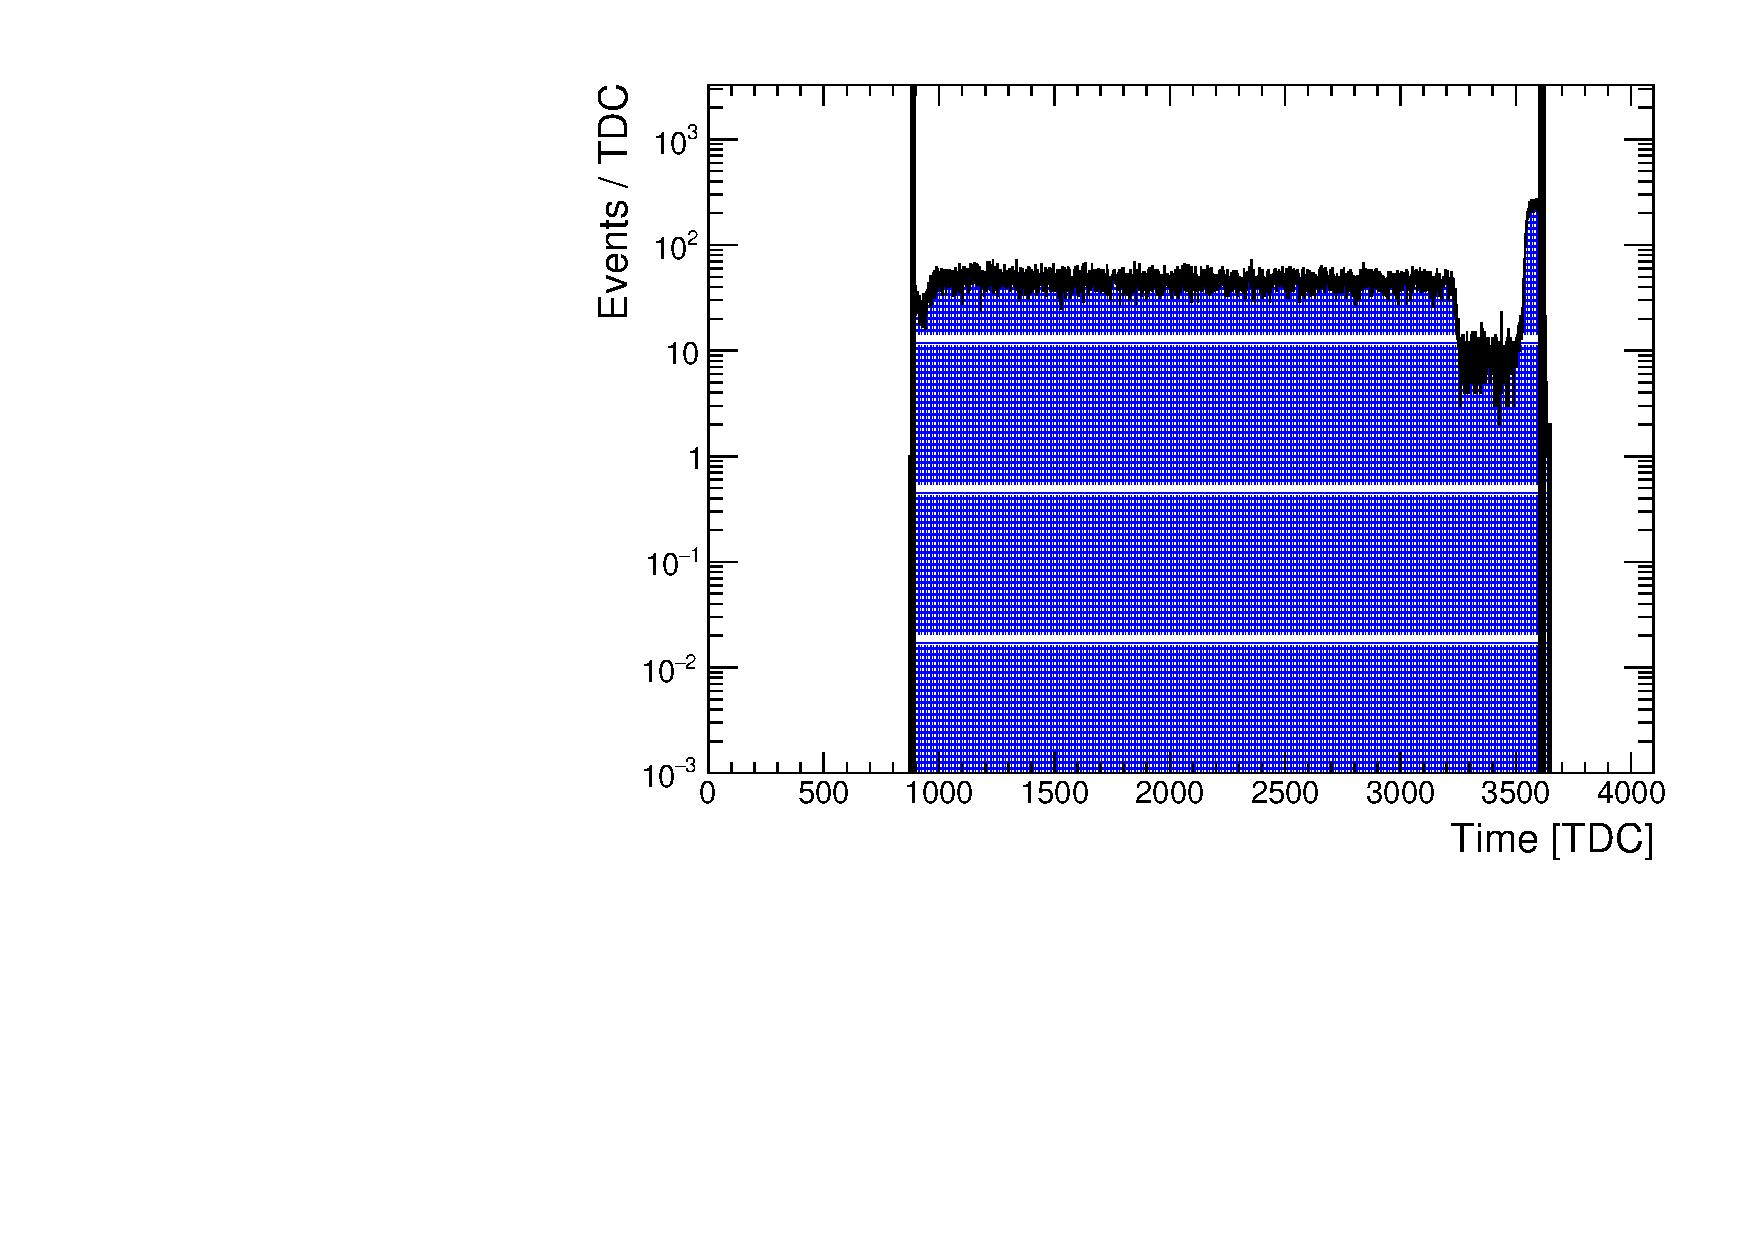
\includegraphics[width=1\linewidth]{../Thesis_Plots/Timing/Muons/Plots/ExampleTDCSpectra.pdf}
		\caption{} \label{fig:TDC_Spectrum}
	\end{subfigure}
	\hfill
	\begin{subfigure}[t]{0.5\textwidth}
		\centering
		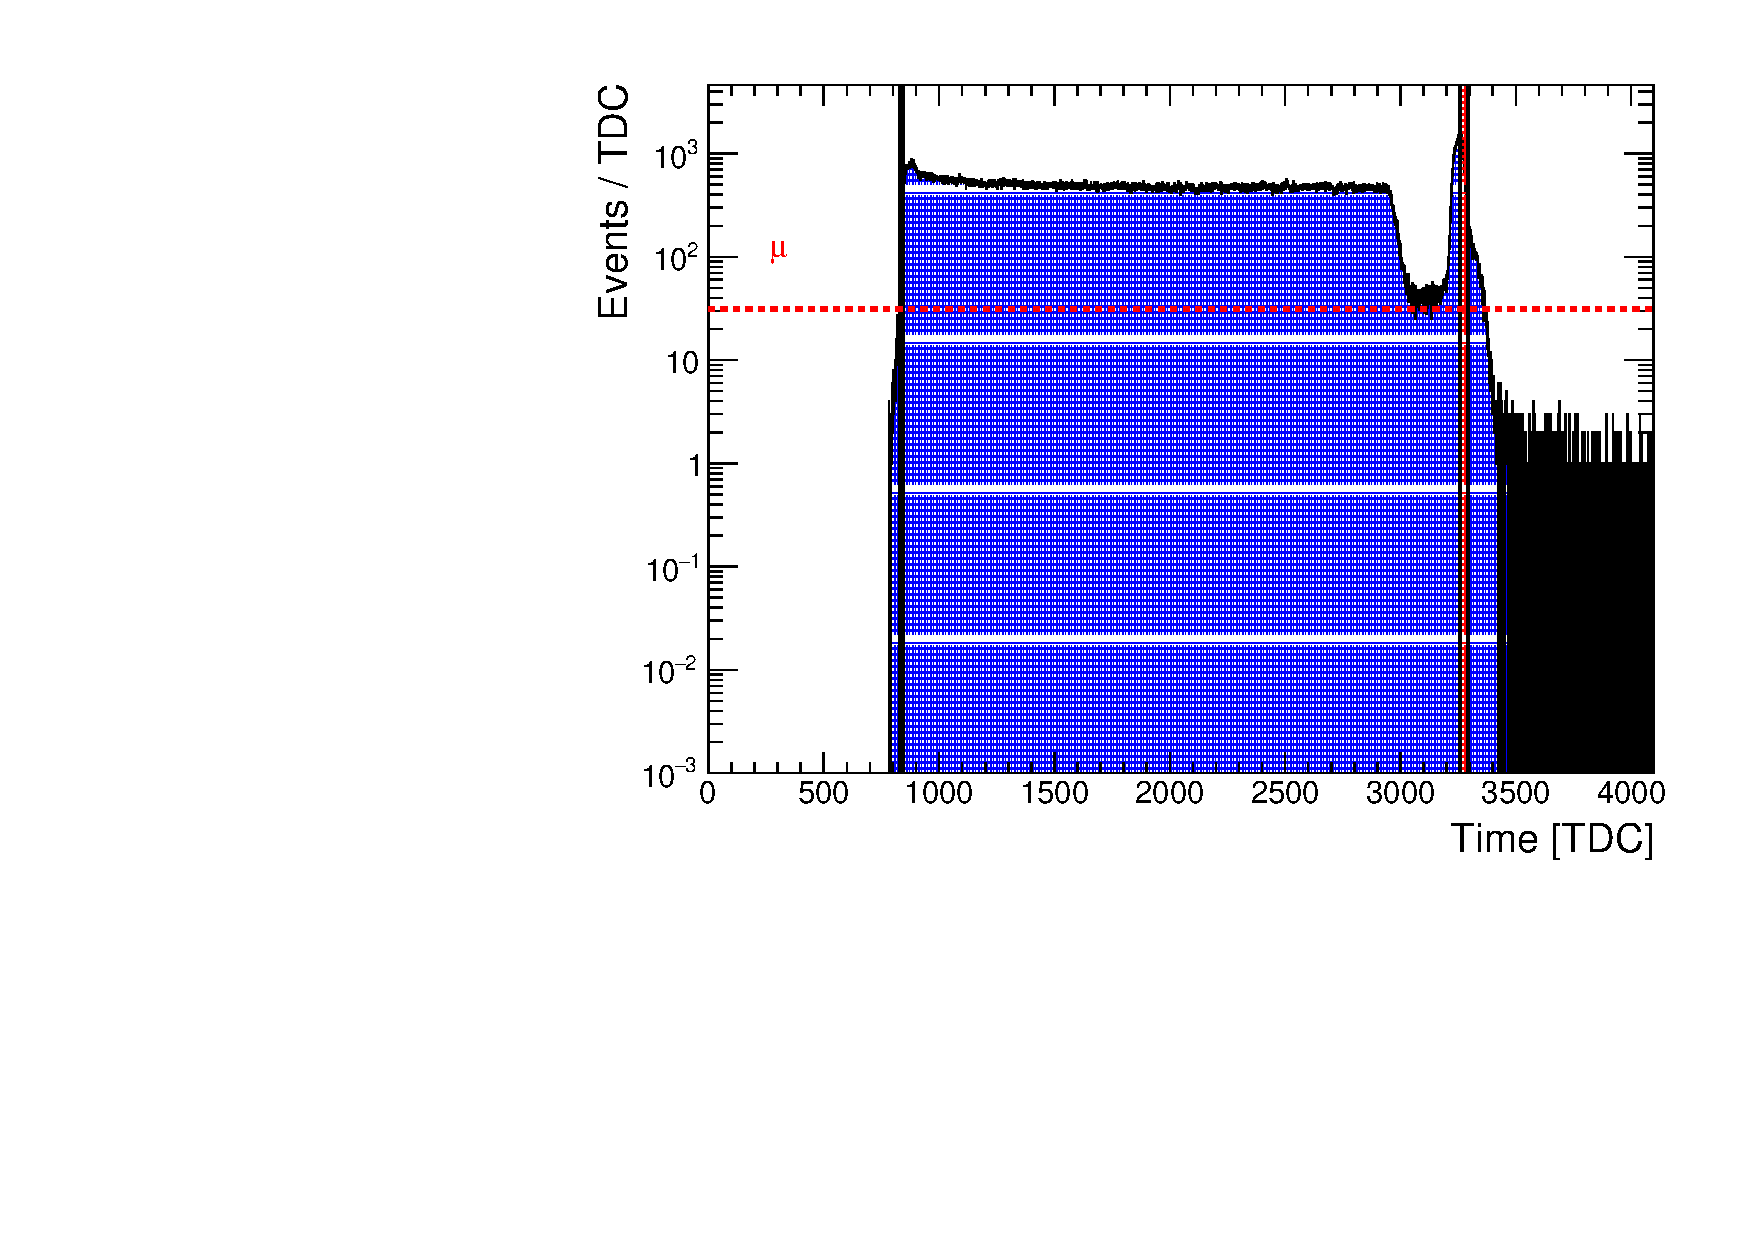
\includegraphics[width=1\linewidth]{../Thesis_Plots/Timing/Muons/Plots/BadTDCSpectra_Layer11.pdf}
		\caption{} \label{fig:TDC_Spectrum_bad}
	\end{subfigure}
	\caption{\subref{fig:TDC_Spectrum}) TDC spectrum of a typical chip. The black lines indicate the fitted Max and Pedestal parameters for this chip. The yellow bands represent the uncertainty on the extraction of the parameter $a$ and $b$. The extracted parameters are $s$ = 1.47 $\pm$ 0.01 ns/TDC, $b$ = 888 $\pm$ 5 TDC and $a$ = 3613 $\pm$ 8 TDC. \subref{fig:TDC_Spectrum_bad}) TDC spectrum of a bad chip on layer 11. The chip 175 on this layer is presenting a long tail to high TDC values. The reason is not understood but present on all chips on that layer.}
\end{figure}

The extraction of the parameters $a$ and $b$ is done by detecting the edges of the TDC spectrum. A threshold $\mu$ is used to extract $a$. This threshold corresponds to the mean of the vertical axis of the TDC spectrum. The parameter $a$ is extracted as the value of the first bin above 30\% of the threshold $\mu$. The endpoint of the ramp is extracted as the value of the last bin above 50\% of the maximum bin content of the TDC spectrum. The start point and the endpoint of the ramp are not extracted as the first and the last bin of the TDC spectrum, because the extraction technique needs to be robust against outliers and strange spectra such as the one shown in figure \ref{fig:TDC_Spectrum_bad}.

An estimation of the uncertainties of the method has been performed. This is done to evaluate the precision of the extraction method. The uncertainty on the parameter $a$ is done by varying the 30\% threshold value by the uncertainty of $\mu$. Similarly for the parameter $b$, the uncertainty is done by varying by 1/3 of the maximum bin content. More details about the estimation of the calibration uncertainties is described in the appendix \ref{appendix:calib_error}.

The extracted values for the slopes are shown in figure \ref{fig:slope_time}. They are in the expected range of 1.6 ns per TDC bin due to the limited dynamic range provided by the chip, around 2500 TDC bins for 4 $\mu$s.

\begin{figure}[htbp!]
	\centering
	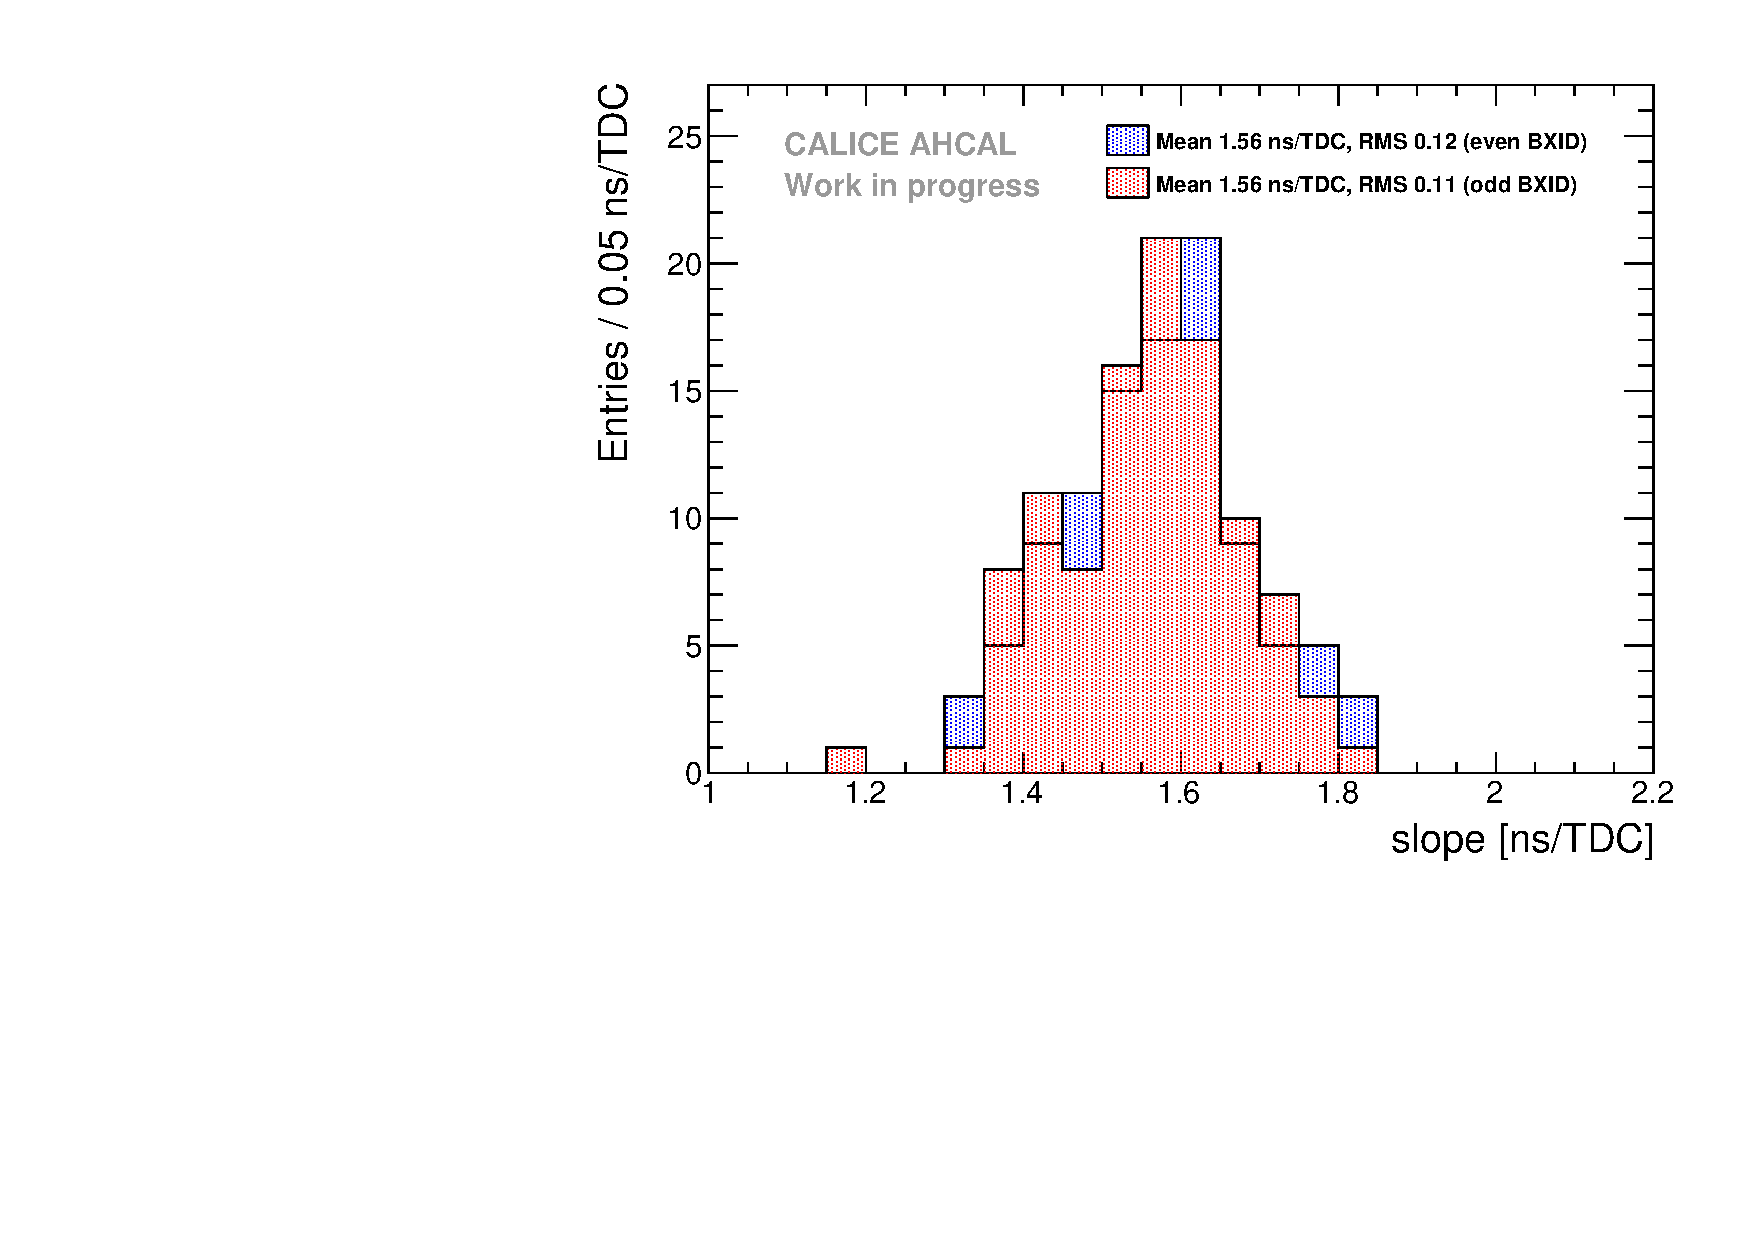
\includegraphics[width=0.5\linewidth]{../Thesis_Plots/Timing/Muons/Plots/SlopesTDC.pdf}
	\caption{Distribution of the fitted slopes for even and odd bunch-crossing IDs. $\mu_{odd}$ = 1.564 ns/TDC, RMS$_{odd}$ = 0.121, $\mu_{even}$ = 1.556 ns/TDC, RMS$_{even}$ = 0.113. In total, 208 TDC slopes were extracted.} \label{fig:slope_time}
\end{figure}

Once the ramp slope has been extracted for each chip and BXID parity, the time of a hit in the i-th channel can then be calculated as
\begin{equation} \label{eq:time_chn}
	t_{i} \: \text{[ns]} = s \times (\text{TDC}_{i} - b)
\end{equation}
where $t_{i}$ is the time of the i-th channel, $s$ is the ramp slope, TDC$_{i}$ is the TDC value of the i-th channel and $b$ is the TDC pedestal value of the i-th channel for the first memory-cell without taking into account the BXID parity. Any time offsets that can be induced by the other memory-cells and the BXID parity can be corrected in a later stage (see section \ref{sec:TimeHit}).

\section{Calibration of the time reference}
\label{section:time_ref}

To reconstruct the time of the first hit in a channel, the measured time of a hit needs to be compared to the time of a reference trigger. The trigger signals described in section \ref{subsec:trigger} are calibrated using the same method as explained above. With the addition that the pedestal value is extracted for all memory cells, possible due to the high statistics, to guaranty the most accurate result.

\begin{figure}[htbp!]
	\begin{subfigure}[t]{0.5\textwidth}
		\centering
		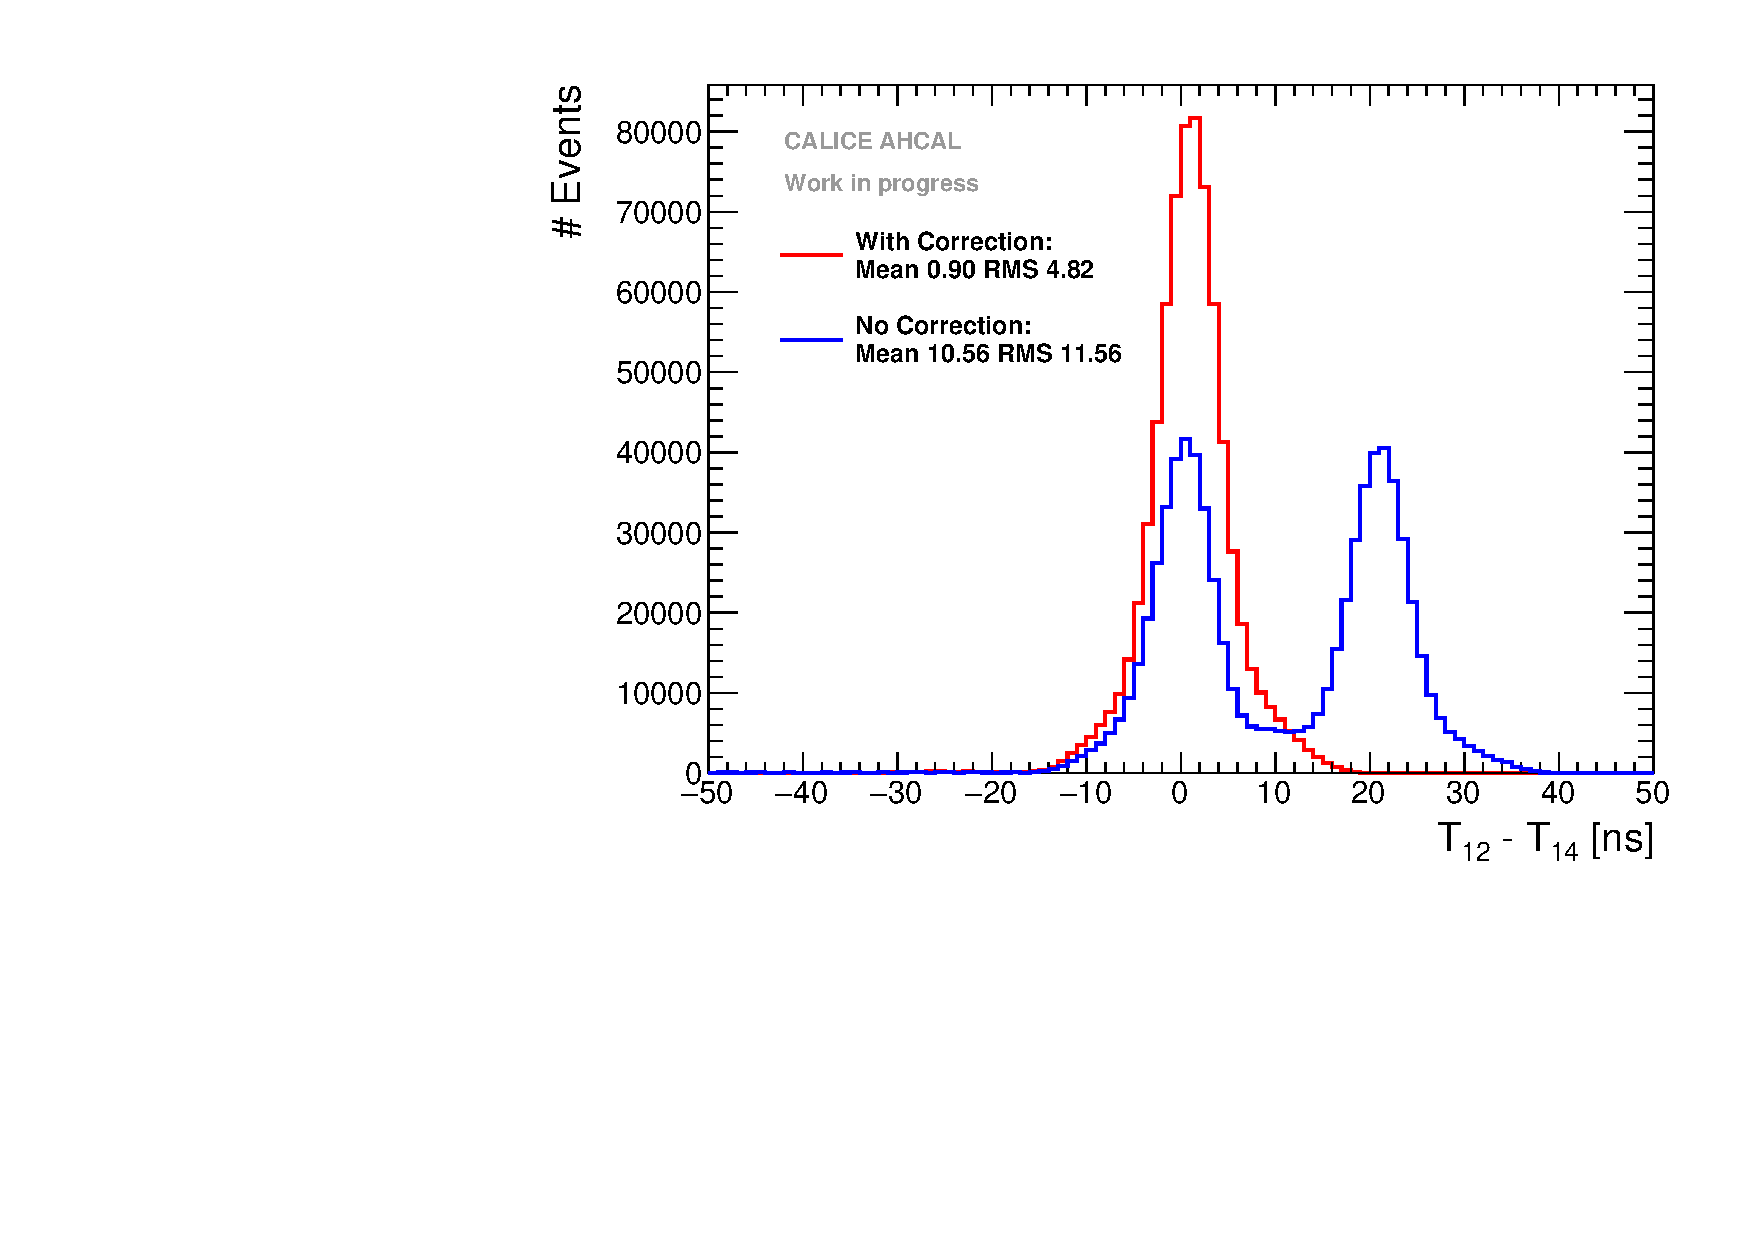
\includegraphics[width=1\textwidth]{../Thesis_Plots/Timing/T0s/Plots/T0_Resolution_5.pdf}
		\caption{Time difference between the trigger channels before and after correction for T$_{12}$ and T$_{14}$.}	\label{fig:T0_Correction}
	\end{subfigure}
	\hfill
	\begin{subfigure}[t]{0.5\textwidth}
		\centering
		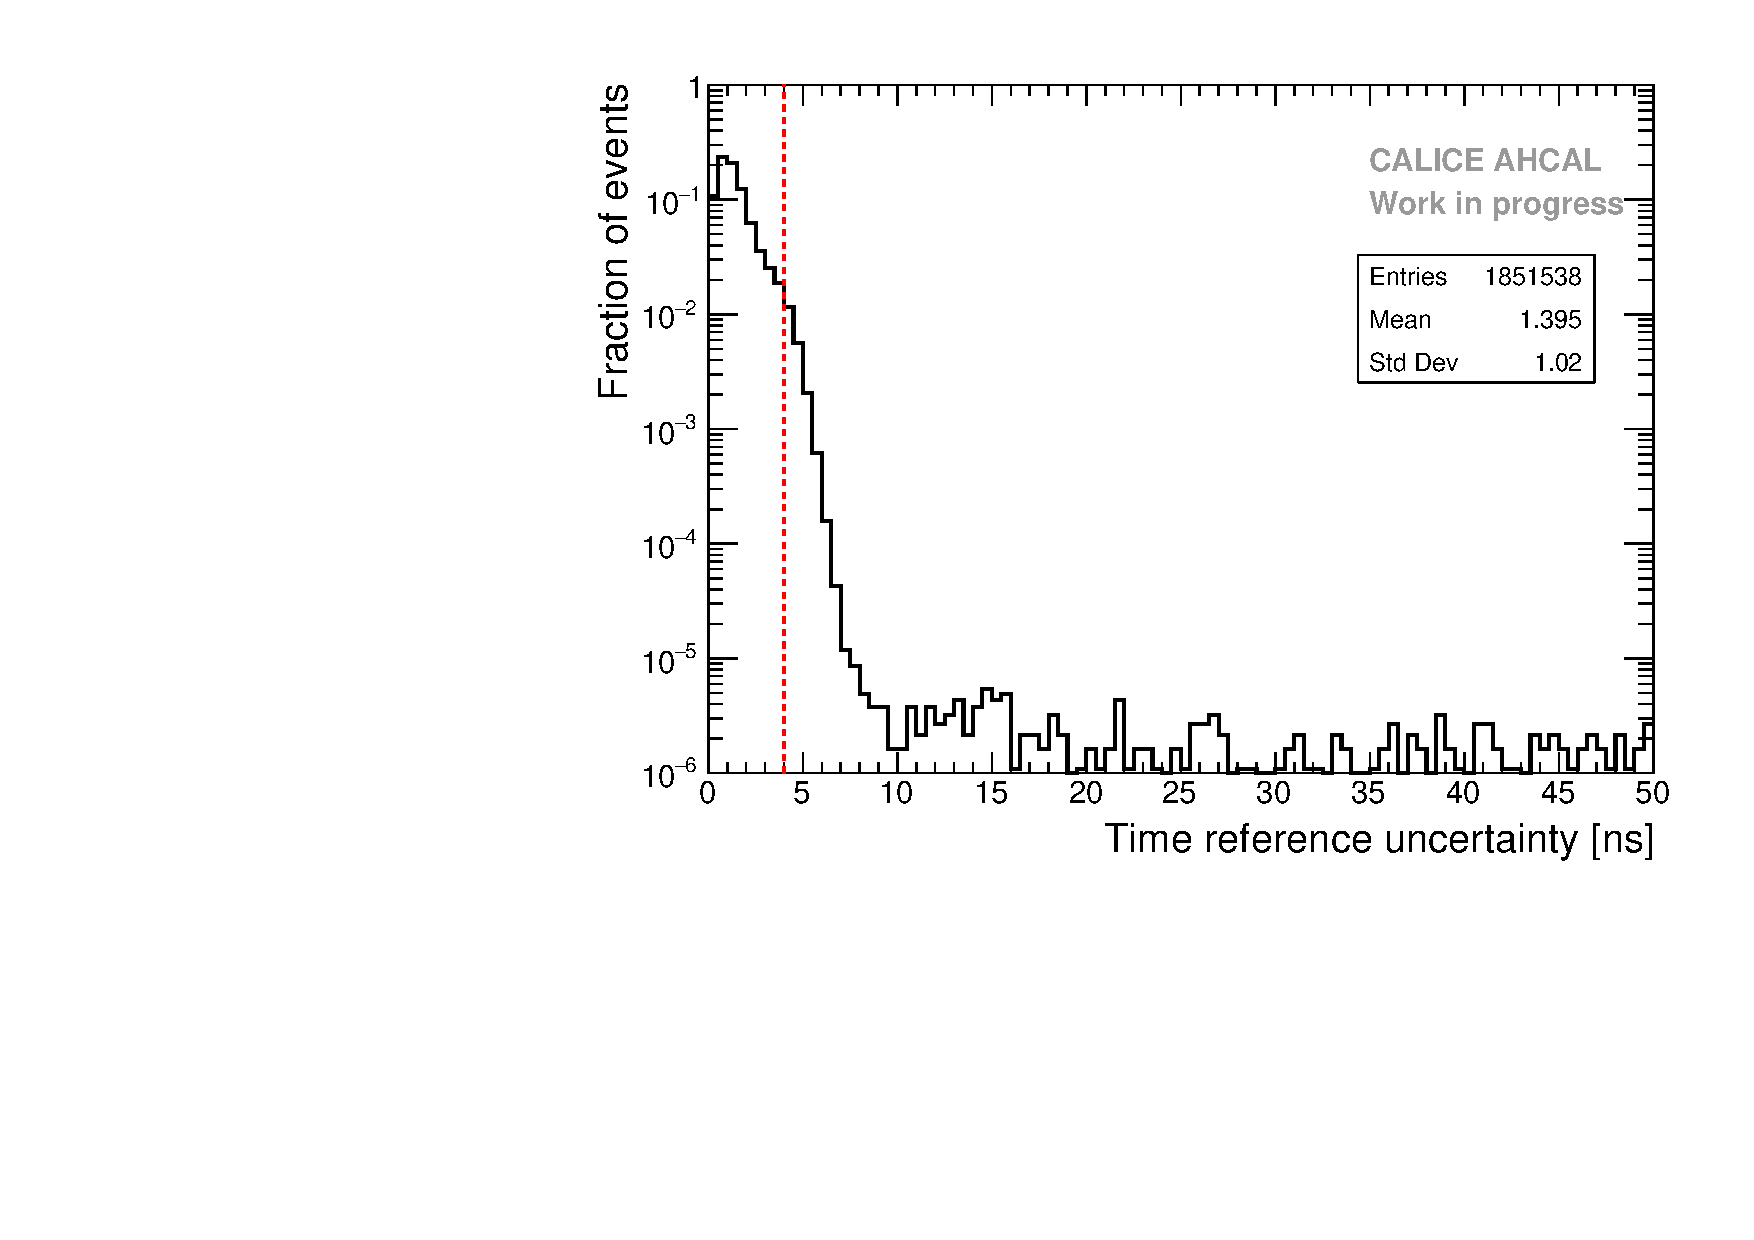
\includegraphics[width=1\linewidth]{../Thesis_Plots/Timing/T0s/Plots/T0ReferenceError}
		\caption{Distribution of the uncertainty $\sigma_{ref}$. The red line represents the cut of 4 ns.} \label{fig:T0ReferenceError}
	\end{subfigure}
	\caption{\subref{fig:T0_Correction}) The histogram in blue shows the difference between the channels before correction, the histogram in red shows the difference after correction. $\mu$ = 10.6 ns, RMS = 11.6 ns, $\mu_{corrected}$ = 0.9 ns, RMS$_{corrected}$ = 4.8 ns. The two visible peaks in blue are due to pedestal values being different dependent of the bunch-crossing parity. \subref{fig:T0ReferenceError}}
\end{figure}

Events are selected by requiring that T$_{12}$, T$_{13}$ and T$_{14}$ are present in the event in a certain amplitude range as shown in table \ref{table:T0_sel} to reject noise hits from these channels. These channels receive the trigger coincidence signal at the same time therefore a correction is applied to ensure that they match in time. This is done to remove any effect induced by the front-end electronics.

A quadratic correction of the time of T$_{12}$ - T$_{14}$ and T$_{13}$ - T$_{14}$ as a function of T$_{12}$ and T$_{13}$ respectively is done. Ideally, the difference between T$_{12}$ and T$_{13}$ to T$_{14}$ should be a Gaussian distribution centered at 0 ns. The figure \ref{fig:T0_Correction} shows the difference T$_{12}$ - T$_{14}$ before correction in blue and after correction in red.

The correction is needed due to the fact that a different value of the pedestal is needed for each BXID parity which was not expected. The resulting RMS of the reference triggers is around 4-5 ns. This resolution from the electronics contributes to the final timing resolution obtained.

\begin{equation} \label{eq:tref}
	\text{T}_{ref} = \frac{\text{T}_{12} + \text{T}_{13} + \text{T}_{14}}{3}
\end{equation}
\begin{equation} \label{eq:tref_err}
	\sigma_{ref}^2 = \frac{ (\text{T}_{12} - \text{T}_{ref})^2 + (\text{T}_{13} - \text{T}_{ref})^2  + (\text{T}_{14} - \text{T}_{ref})^2 }{6}
\end{equation}

In a next step, to reduce the uncertainty of the time reference, the time reference $T_{ref}$ and its associated uncertainty $\sigma_{ref}$ are calculated following the equations \ref{eq:tref} and \ref{eq:tref_err}. A cut of 4 ns is performed on $\sigma_{ref}$ to reject events with a too large uncertainty on the time of the trigger reference as shown in figure \ref{fig:T0ReferenceError}. The mean uncertainty of the time reference is around 1.30 ns which is compatible with previous results \cite{Laurien2016}. Finally, only events with a calibrated time value between 500 and 3500 ns were considered to avoid TDC ramp edge effects.

\section{Determination of the time of the first hit}
\label{sec:TimeHit}

Due to cabling and the trigger electronics logic, the time reference is delayed compared to the muon passing through the detector. Therefore, the time offset of the time reference is determined from data. Muons are instantaneous particles thus the time of the first hit distribution for each channel, memory cell and BXID should peak at 0 ns.

A shifting procedure of the time of the hit relative to the time reference for each channel, memory-cell and BXID parity is performed. This is done to take into account the delay time of the trigger due to cabling and the NIM-logic as well as possible differences in pedestals. Only memory-cells containing more than 100 events are considered. The histogram range of the time of the hit relative to the time reference is reduced iteratively until the RMS of the distribution is under 10 ns. This value was arbitrary chosen. The mean of the histogram is then used as the time offset value. An example of a single channel is shown in figure \ref{fig:TimeChnwithOffset}.

\begin{figure}[htbp!]
	\begin{subfigure}[t]{0.5\textwidth}
		\centering
		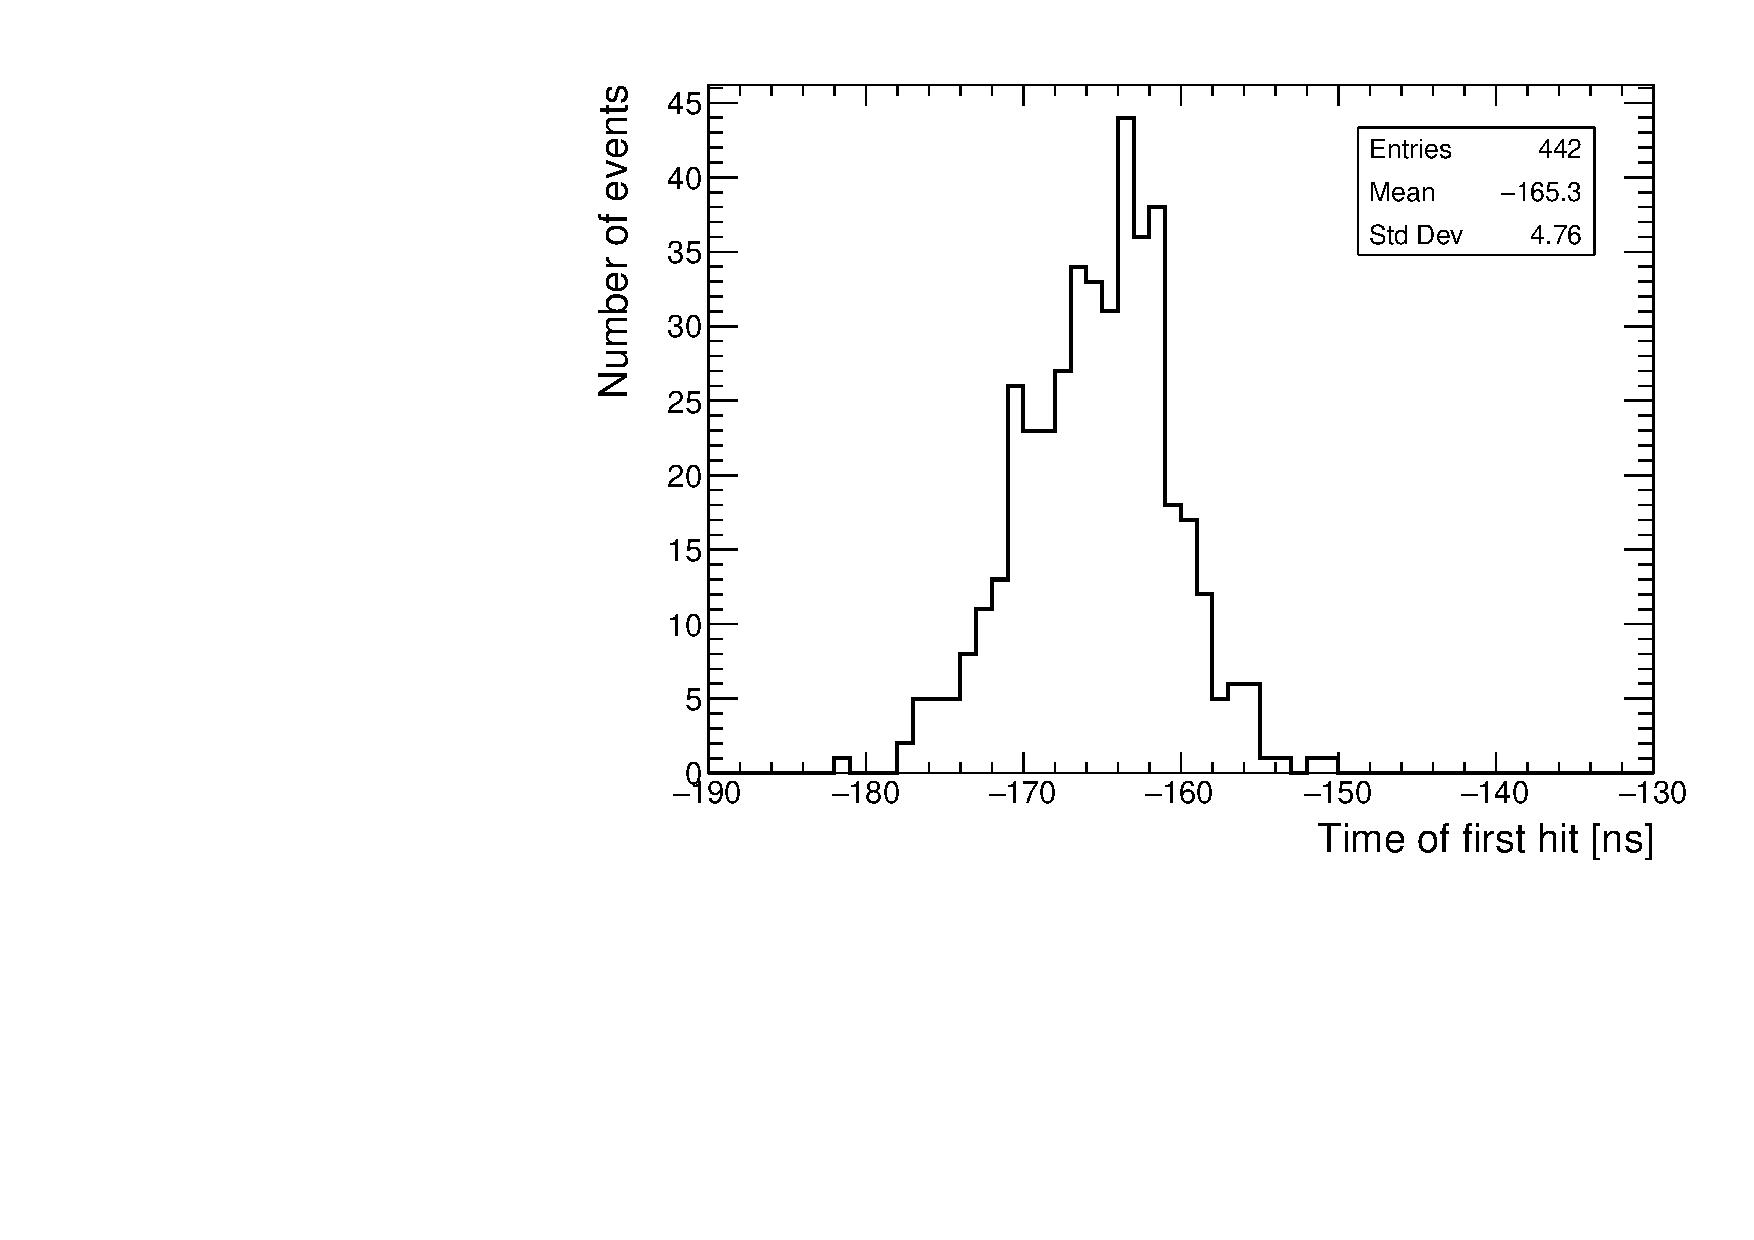
\includegraphics[width=1\textwidth]{../Thesis_Plots/Timing/Muons/Plots/Timing_Chip236_Chn21_Mem01_BXID1_withOffset.pdf}
		\caption{}\label{fig:TimeChnwithOffset}
	\end{subfigure}
	\hfill
	\begin{subfigure}[t]{0.5\textwidth}
		\centering
		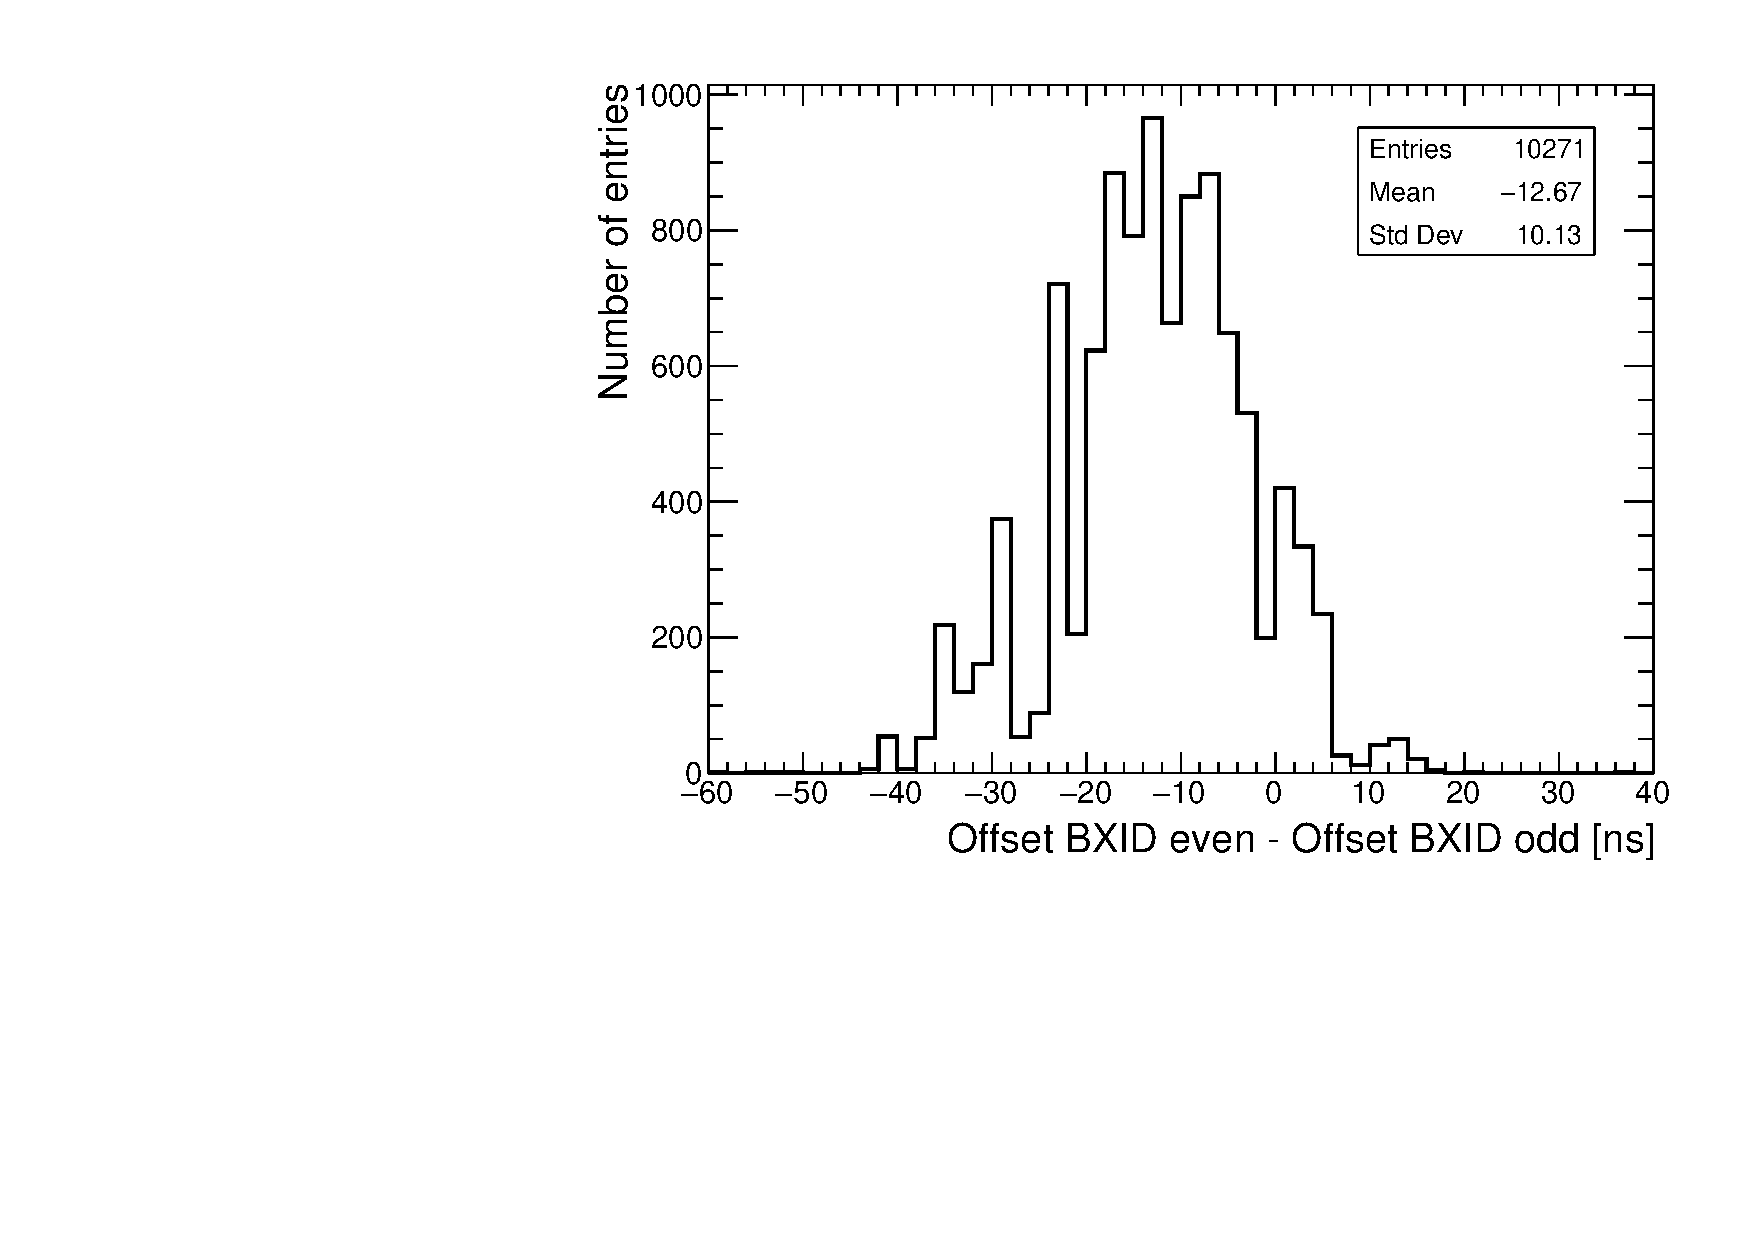
\includegraphics[width=1\textwidth]{../Thesis_Plots/Timing/Muons/Plots/BXIDDifferenceOffsets.pdf}
		\caption{}\label{fig:BXID_offset}
	\end{subfigure}
	\caption{\subref{fig:TimeChnwithOffset}) Time of first hit distribution for a single channel (Chip 236, Chn 21, Mem 01, BXID 1). An offset of -165.2 ns is determined for this channel. \subref{fig:BXID_offset}) Distribution of the difference of offsets extracted for even and odd BXID for each channel and memory-cell. A mean time offset difference of 12 ns is visible between even and odd BXID.}
\end{figure}

Then a second step is done to account for a possible mis-calibration in the first step of determining the offset. Non-prompt events are tagged by requiring at least 4 prompt hits in the range of -20 to 20 ns. This was necessary in order to reduce the impact of noise and ensure a good calibration of the time offset. Then the time offset is extracted using the same method as described above with the non-prompt events removed.

In total, 21040 individual offsets are extracted from data. The mean value of the time offset is around -150 ns which is in the expected order considering the cabling length and the trigger logic delay. Individual offsets have to be extracted for each BXID parity and memory-cell for the pedestal as shown in figure \ref{fig:BXID_offset}.

\subsection{Time of the first hit distribution}

After calibration, the time of the first hit can be obtained by looking at the distribution of T$_{chn}$ - T$_{ref}$ as shown in figure \ref{fig:timing_nocorrection}. The time resolution (RMS) shown in figure \ref{fig:timing_nocorrection} obtained by combining all layers excluding layer 11 is around 5.65 ns by just applying the time calibration on the data. This is far from the desired time resolution of 1 ns. In addition, an asymmetry can be seen in the time distribution to the left. Some improvements are still possible as described in the following section.

Each layer was looked at individually as shown in figure \ref{fig:reso_nocorrection}. A comparison between a Gaussian fit to extract the $\sigma$ and the RMS of the time distribution is done. All layers are very similar in terms of time resolution and Gaussian-like. The layer 6 and 10 present a higher time resolution that may be due to the bad quality of these boards. The discrepancy observed for the layer 11 is most likely due to an electronic problem in the TDC voltage ramp of all the chips on that layer. All calibration values, channel-wise and chip-wise time distributions on this layer have been investigated manually and all channels present a large tail to high time value. The reason is not clear and identified.

\begin{figure}[htbp!]
	\begin{subfigure}[t]{0.5\textwidth}
		\centering
		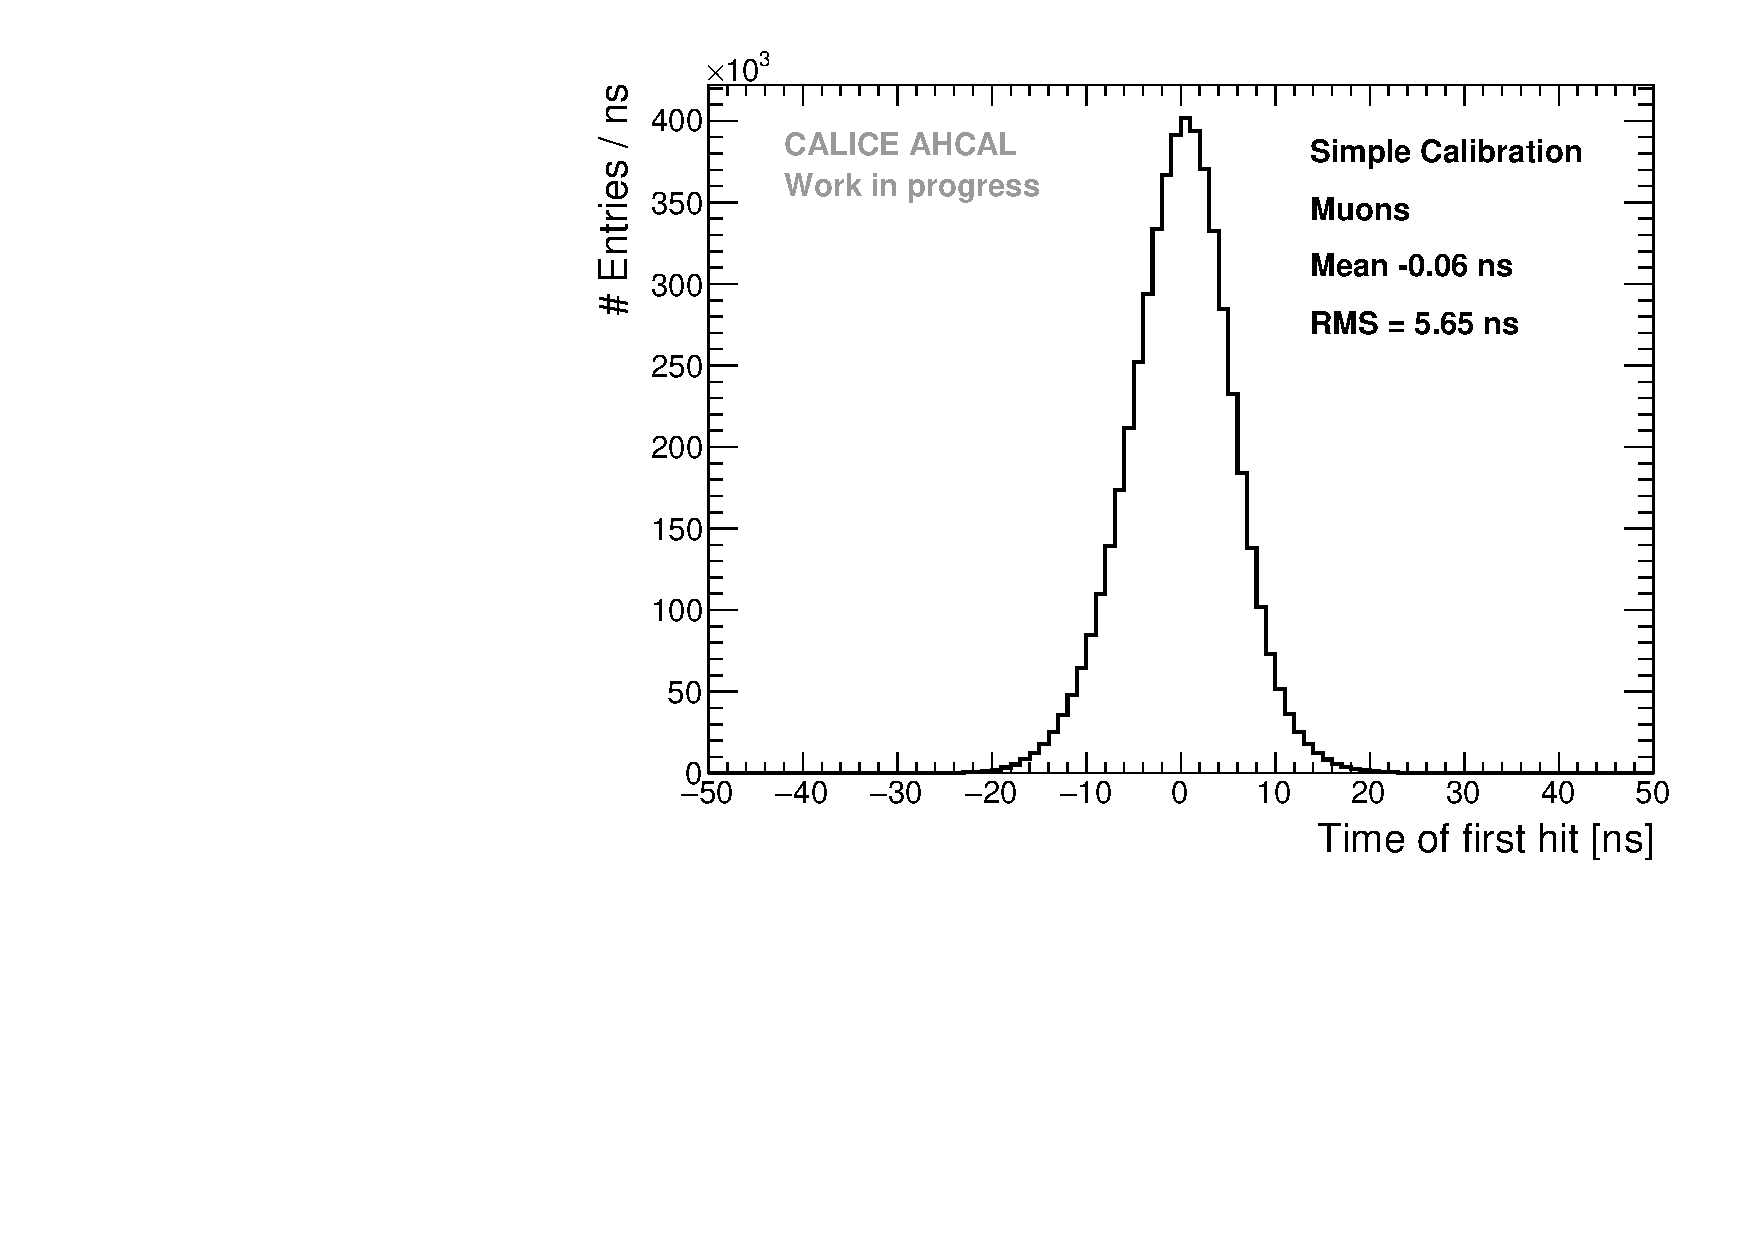
\includegraphics[width=1\textwidth]{../Thesis_Plots/Timing/Muons/Plots/Timing_AHCAL_noCorrections.pdf}
		\caption{}\label{fig:timing_nocorrection}
	\end{subfigure}
	\hfill
	\begin{subfigure}[t]{0.5\textwidth}
		\centering
		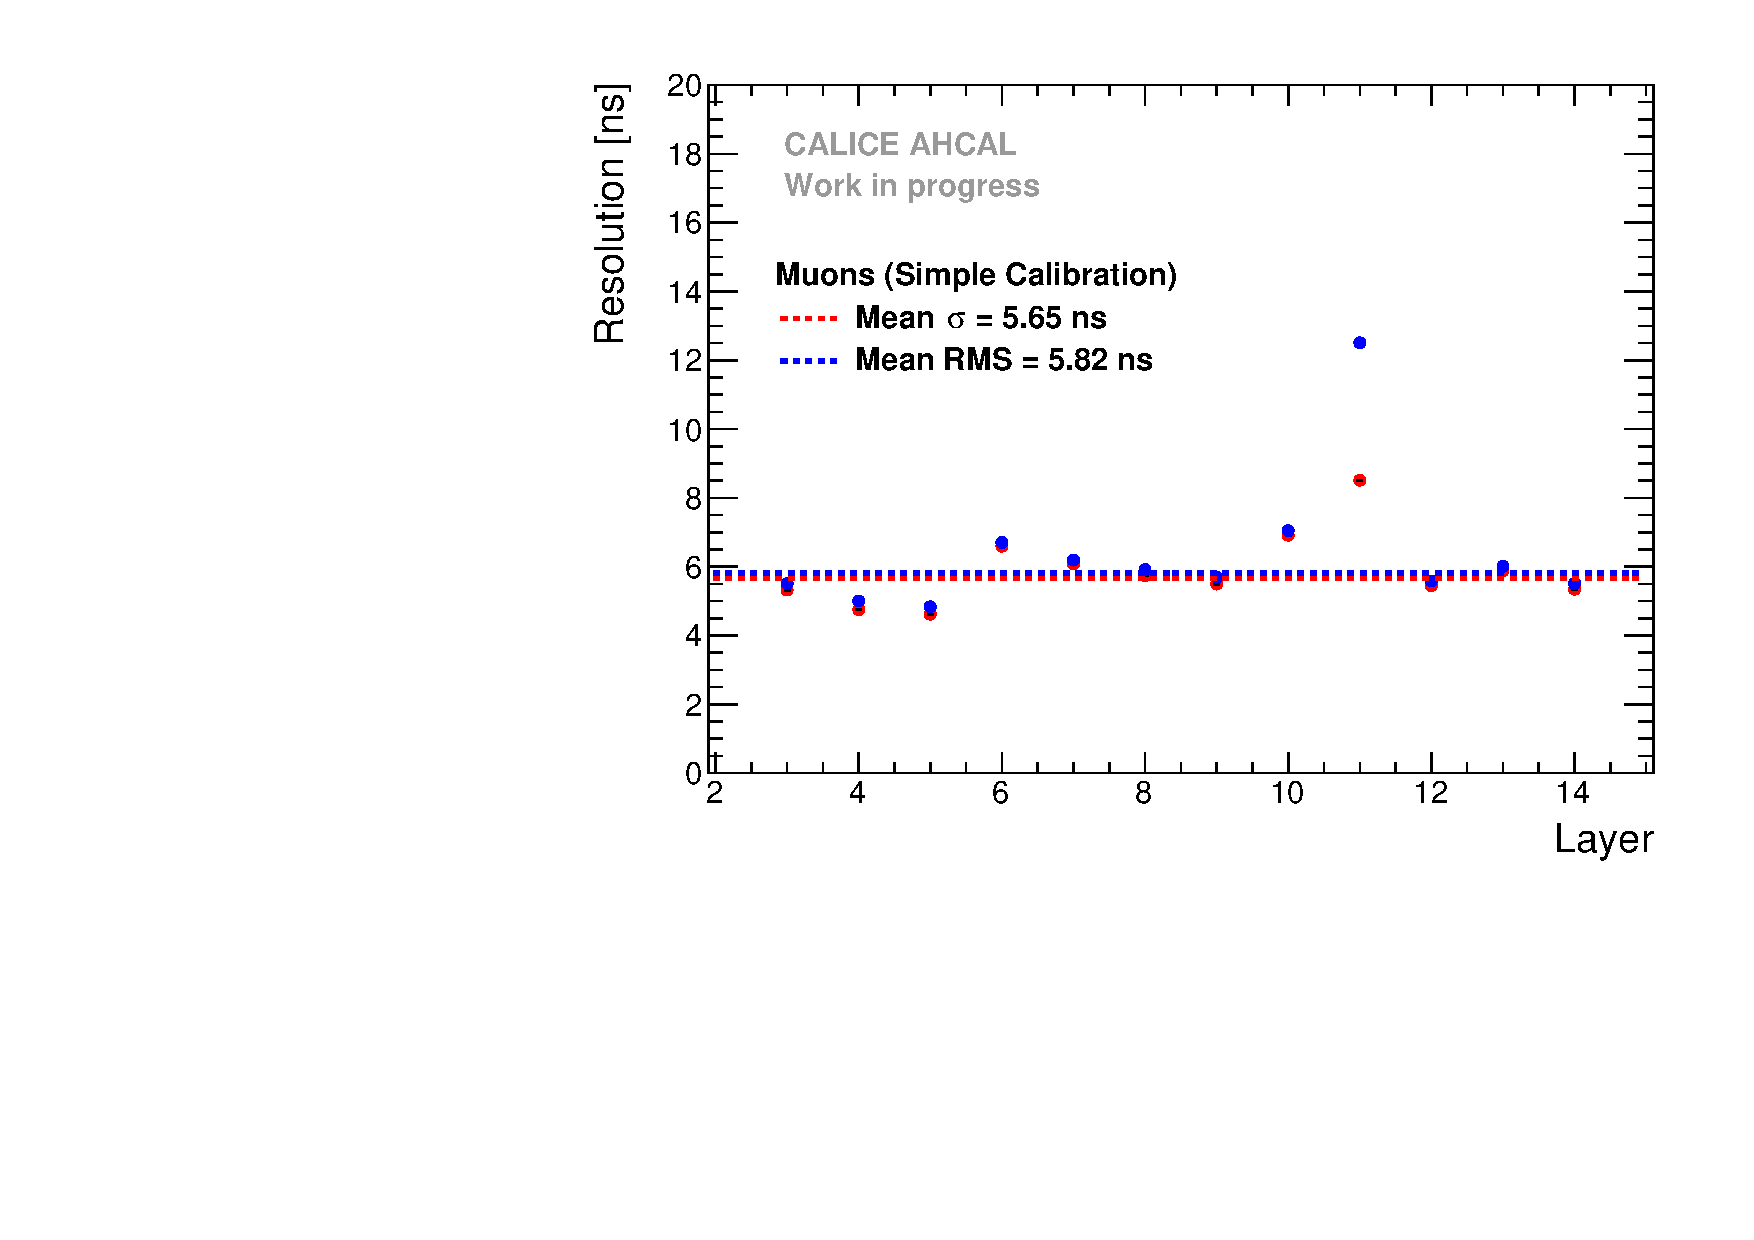
\includegraphics[width=1\textwidth]{../Thesis_Plots/Timing/Muons/Plots/ResolutionPerModule_noCorrections.pdf}
		\caption{}\label{fig:reso_nocorrection}
	\end{subfigure}
	\caption{\subref{fig:timing_nocorrection}) Time of the first hit distribution of the AHCAL after the first part of the calibration. $\mu$ = -0.06 ns , RMS = 5.65 ns. The distribution is asymmetric to the left. \subref{fig:reso_nocorrection}) Time resolution for all layers in the AHCAL. The mean RMS time resolution is represented by the blue line. Mean $\sigma$ = 5.65 ns, Mean RMS = 5.82 ns.}
\end{figure}

\section{Corrections applied to data}

\subsection{Ramp non-linearity correction}
\label{subsec:lin_corr}

The calibration relies on the linearity of the TDC voltage ramp in the \textit{SPIROC2B} by measuring the minimum and maximum of the TDC ramp and determining the slope assuming a linear ramp. This assumption is not entirely reliable as described in \cite{Hartbrich2011, Brianne2012}. The voltage slope shows a slight kink around the middle thus leading to a non-linear ramp. For this, a correction of the non-linearity is applied. Since the time reference is determined from a non-linear TDC ramp and it can't be corrected due to the lack of external time reference, the position of $T_{hit}$ - $T_{ref}$ on the ramp is actually corrected here.

\begin{figure}[htbp!]
	\begin{subfigure}[t]{0.5\textwidth}
		\centering
		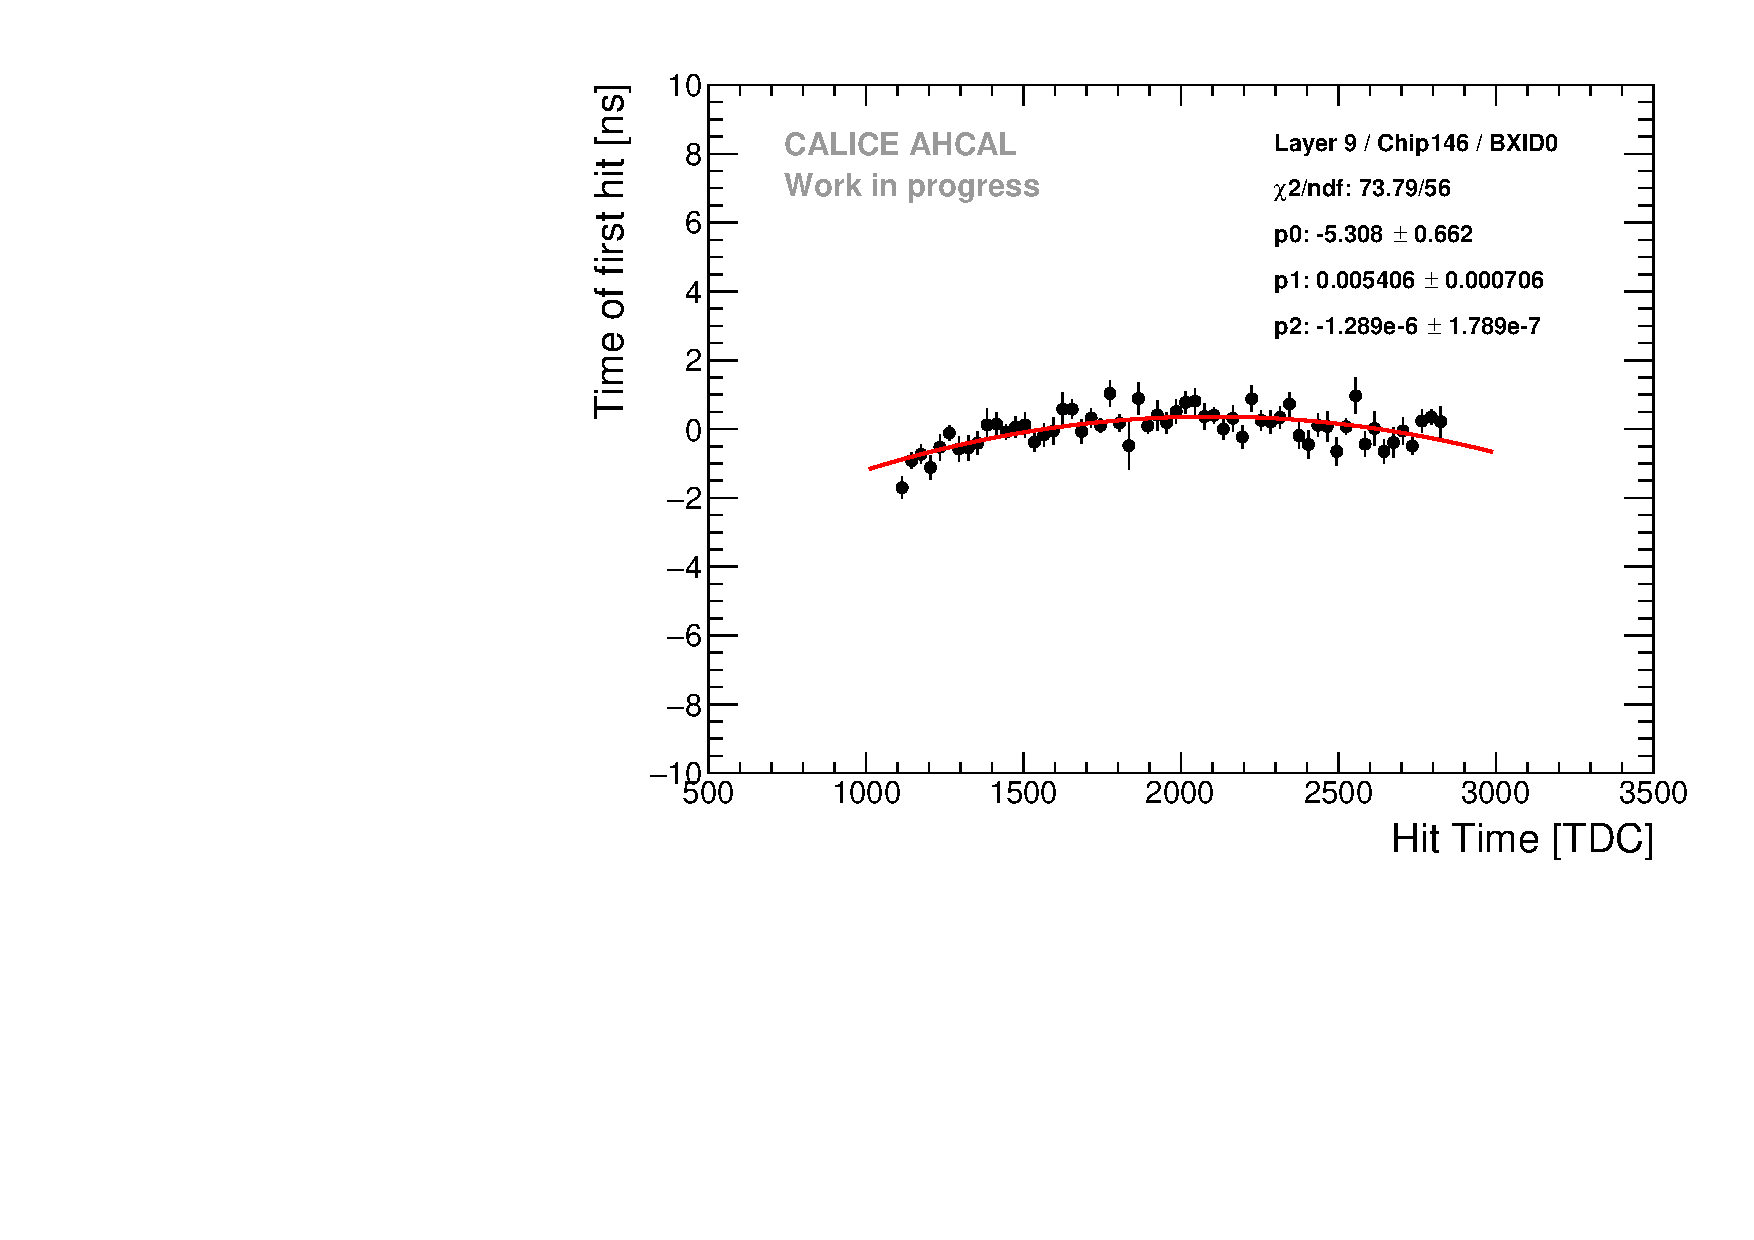
\includegraphics[width=1\textwidth]{../Thesis_Plots/Timing/Muons/Plots/LinearityCorrection_Module09_Chip146_BXID0.pdf}
		\caption{}\label{fig:LinCorr}
	\end{subfigure}
	\hfill
	\begin{subfigure}[t]{0.5\textwidth}
		\centering
		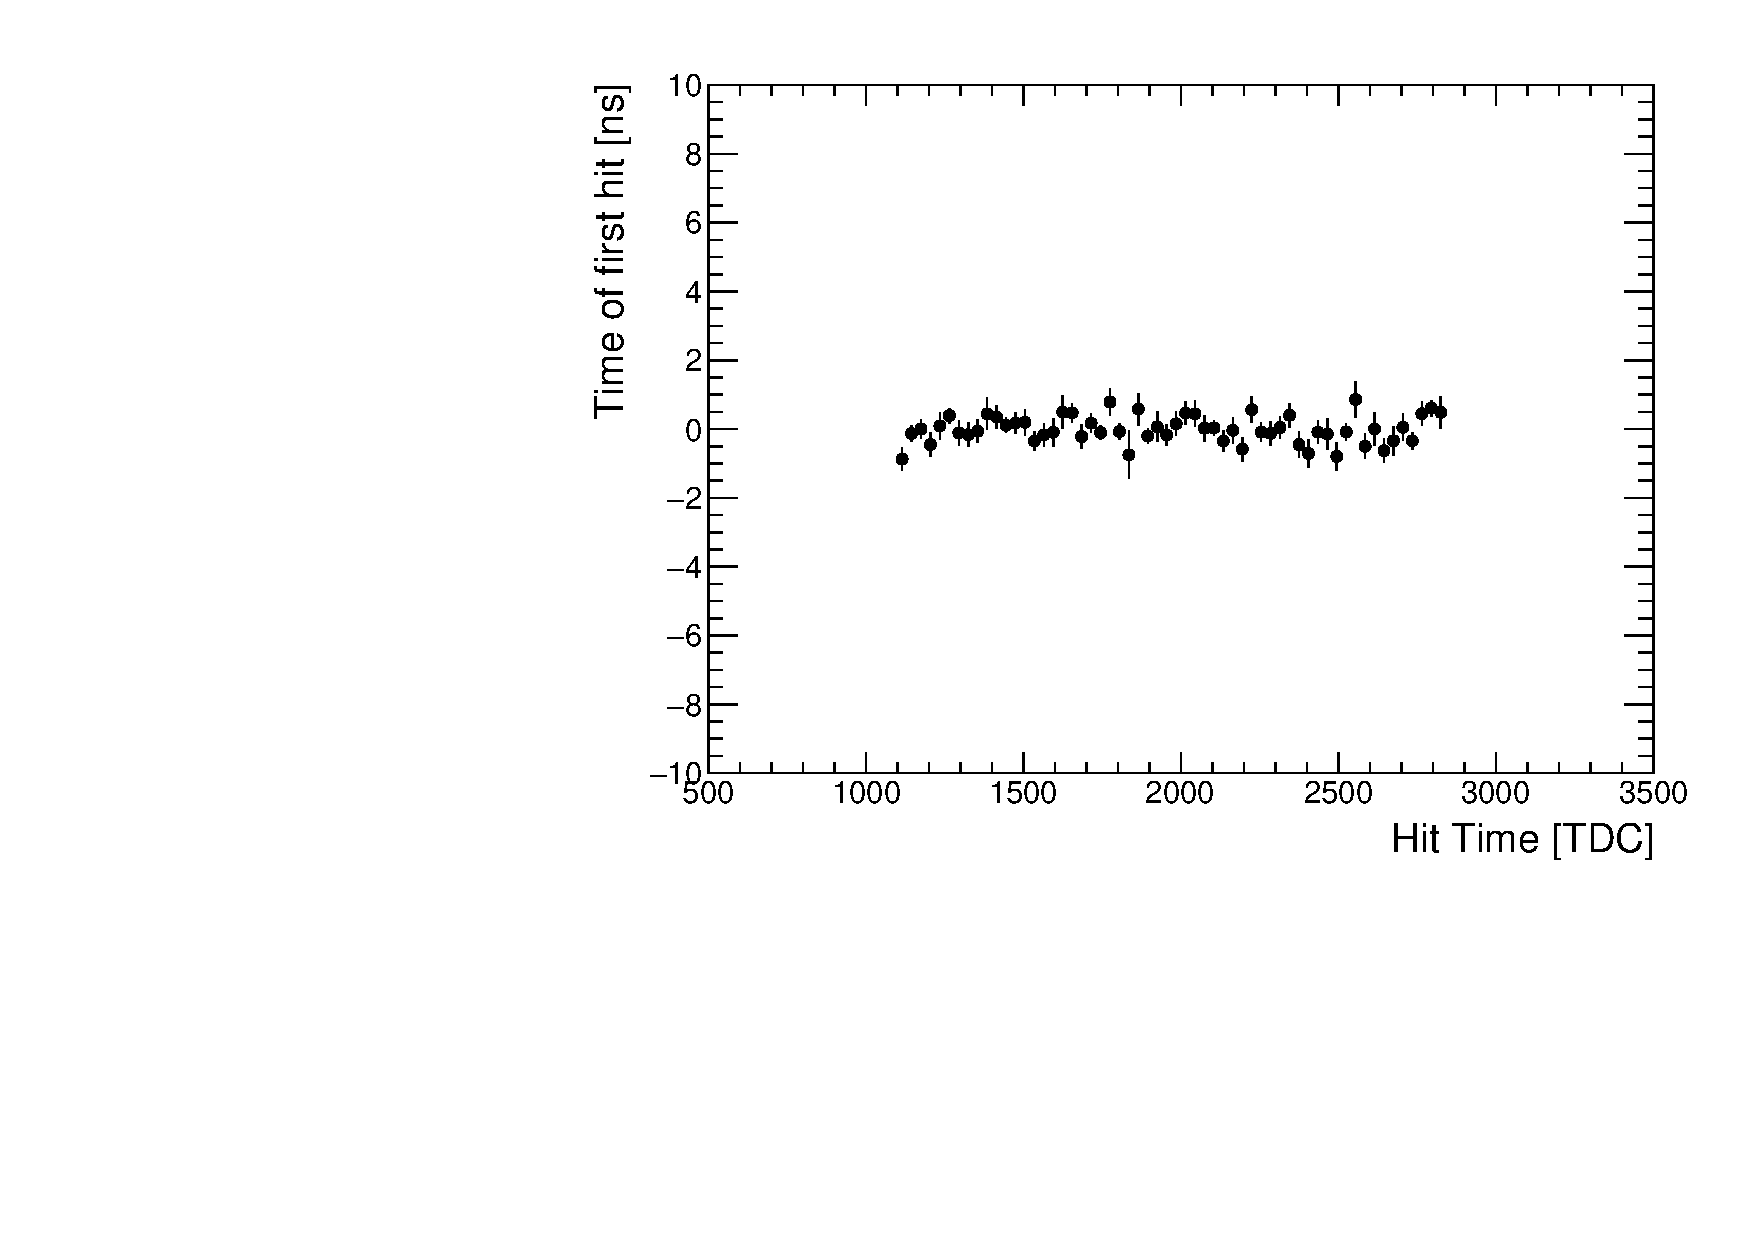
\includegraphics[width=1\textwidth]{../Thesis_Plots/Timing/Muons/Plots/LinearityCorrection_Module09_Chip146_BXID0_Corrected.pdf}
		\caption{}\label{fig:LinCorr_2}
	\end{subfigure}
	\caption{\subref{fig:LinCorr}) Quadratic fit of chip 146 (BXID even) on layer 9. The graph is slightly curved showing that this chip presents a non-linear TDC ramp. $\chi^2/ndf$ = 1.29. \subref{fig:LinCorr_2}) Profile for chip 146 on layer 9 after the non-linearity correction of the ramp. The correction parameters are applied on the data to cross-check the quality of the correction. The curve flattens with the non-linearity correction applied.}
\end{figure}

By investigating the time of the first hit (T$_{fH}$) for each chip and BXID parity as a function of the TDC value of the hit, the shape of the graph indicates how reliable is the assumption of a linear ramp. If the ramp would be perfectly linear, one would obtain a flat graph. To correct for the non-linearity of the ramp, a quadratic fit is performed for each chip and \acrshort{bxid} as shown in figure \ref{fig:LinCorr}. The correction needed can be in the order of few nanoseconds. The figure \ref{fig:LinCorr_2} shows the time of first hit as a function of the TDC value of the hit after the non-linearity correction. The curve looks much flatter.

The non-linearity correction results in an improvement in the timing resolution (RMS) of the AHCAL by about 5.1\% (from 5.65 to 5.36 ns) as shown in figure \ref{fig:timing_lincorrection}. Looking at each layer, as shown in figure \ref{fig:reso_lincorrection}, the time resolution went down by the same amount.

\begin{figure}[htbp!]
	\begin{subfigure}[t]{0.5\textwidth}
		\centering
		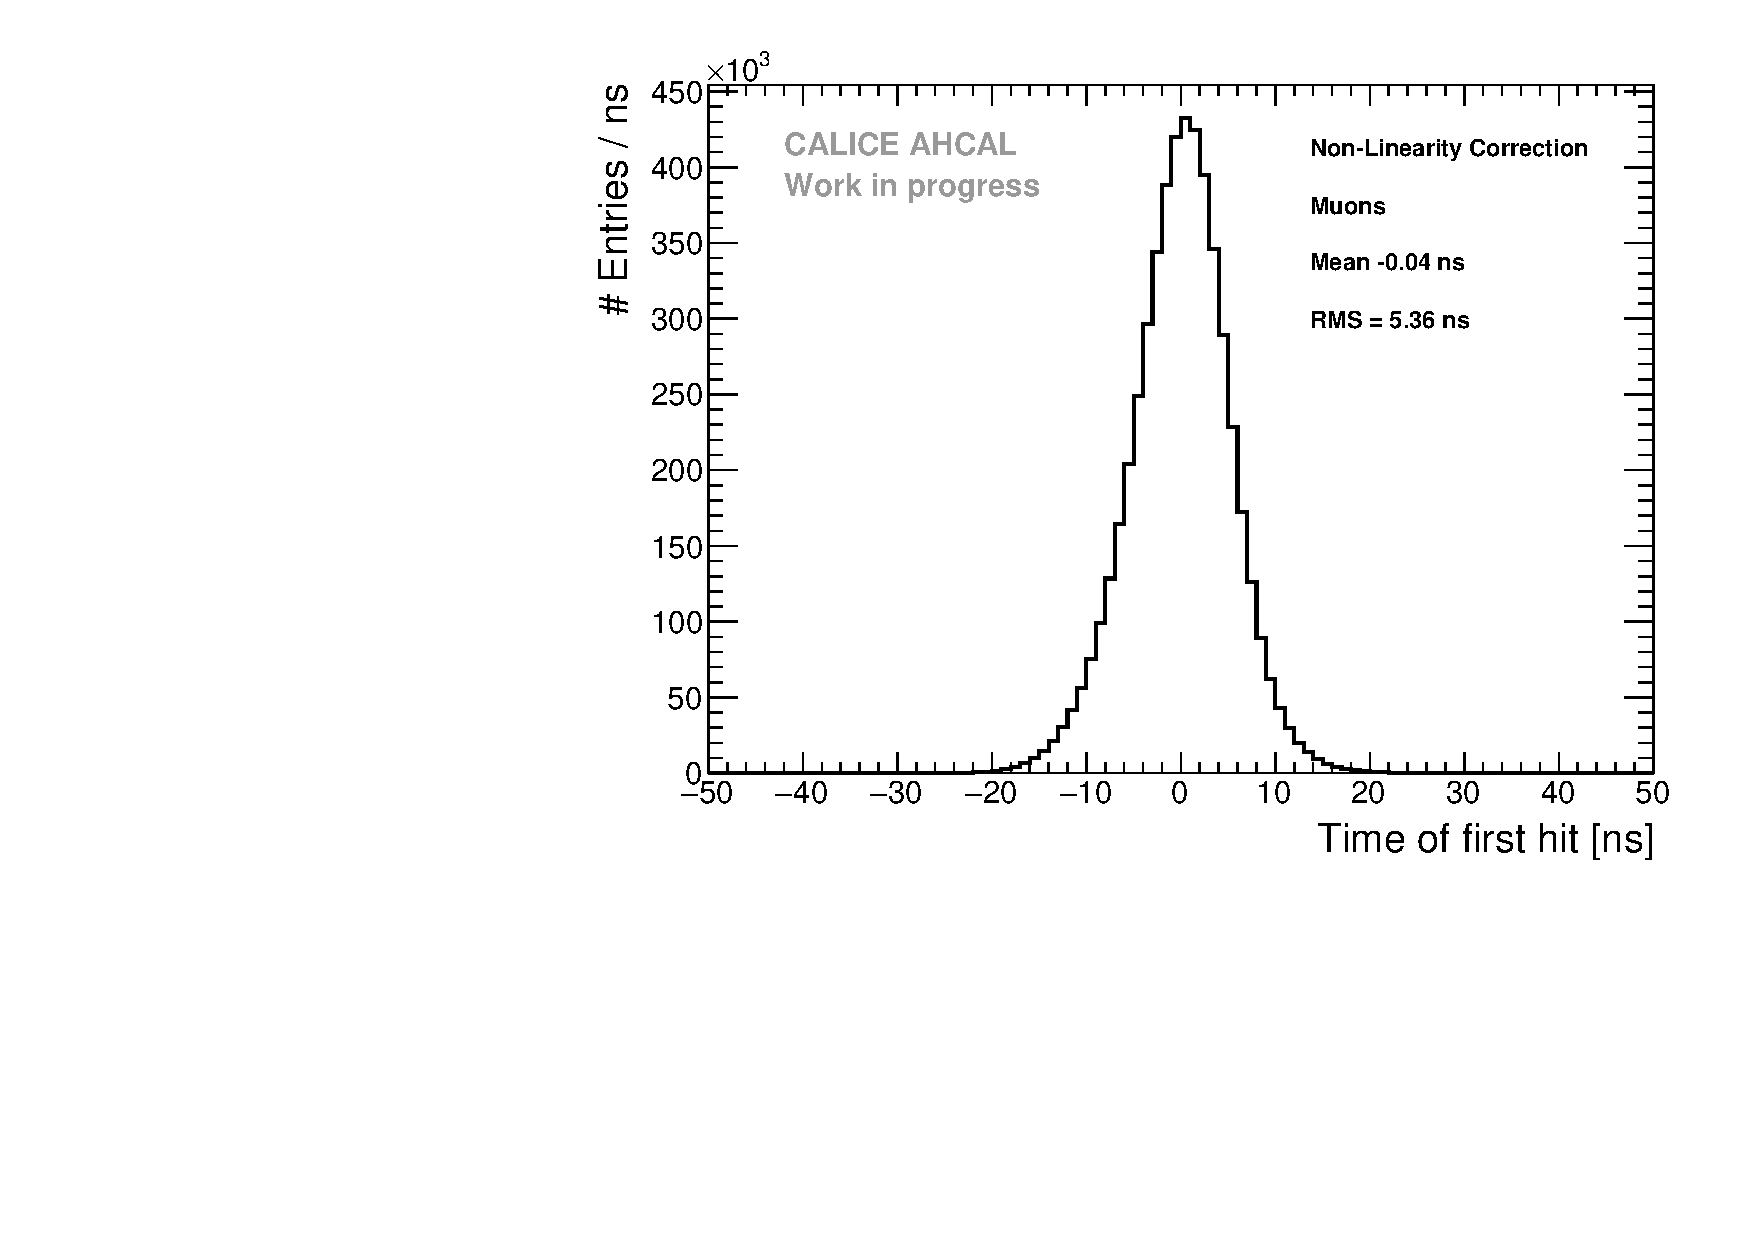
\includegraphics[width=1\textwidth]{../Thesis_Plots/Timing/Muons/Plots/Timing_AHCAL_LinCorrection.pdf}
		\caption{}\label{fig:timing_lincorrection}
	\end{subfigure}
	\hfill
	\begin{subfigure}[t]{0.5\textwidth}
		\centering
		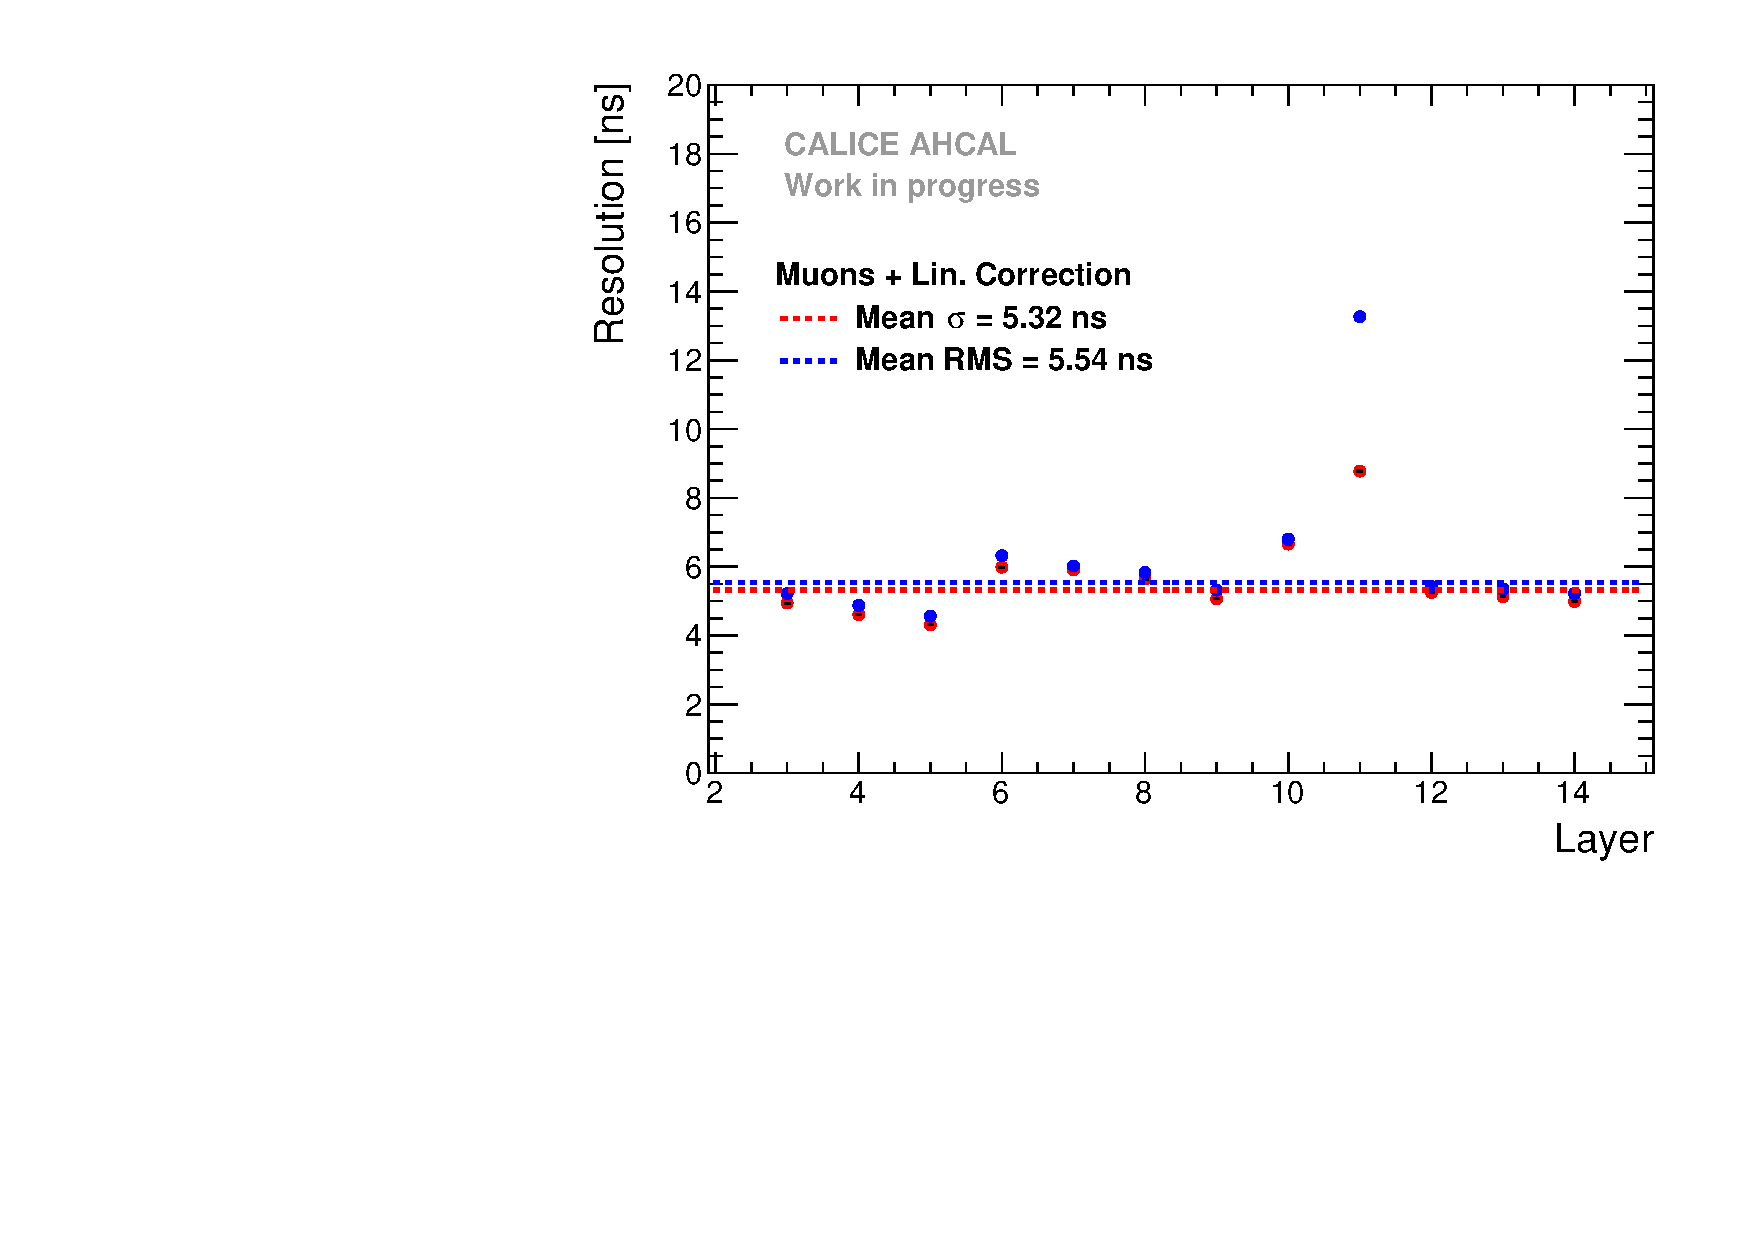
\includegraphics[width=1\textwidth]{../Thesis_Plots/Timing/Muons/Plots/ResolutionPerModule_LinCorrection.pdf}
		\caption{}\label{fig:reso_lincorrection}
	\end{subfigure}
	\caption{\subref{fig:timing_lincorrection}) Time of the first hit distribution of the AHCAL after the non-linearity correction. $\mu$ = -0.04 ns , RMS = 5.36 ns. \subref{fig:reso_lincorrection}) Time resolution for all layers in the AHCAL. The mean RMS is 5.54 ns.}
\end{figure}

However, the asymmetry of the time distribution remains. This effect has been investigated and appears for all layers and chips. It may be due to the time reference channels because the non-linearity of the TDC ramp for these channels can not be corrected without an external time reference. This has been investigated by looking at the time of first hit distribution in bins of the mean TDC value of the time reference. It has been observed, for all layers, that the time asymmetry increases as a function of the TDC value of the time reference.

\subsection{Time Walk correction}
\label{subsec:timewalk}

The time-walk effect is due to the presence of a threshold that induces a time shift between a small amplitude signal and a high amplitude signal. Small amplitude signals will systematically trigger at a later time than high amplitude signals for a shaper that makes the signals peak at the same time. A correction can be determined by looking at the time of the first hit as a function of the amplitude of the hit. This may be particularly important for late neutrons energy depositions in hadron showers that generally deposit very little energy in the calorimeter.

\begin{figure}[htbp!]
	\begin{subfigure}[t]{0.5\textwidth}
		\centering
		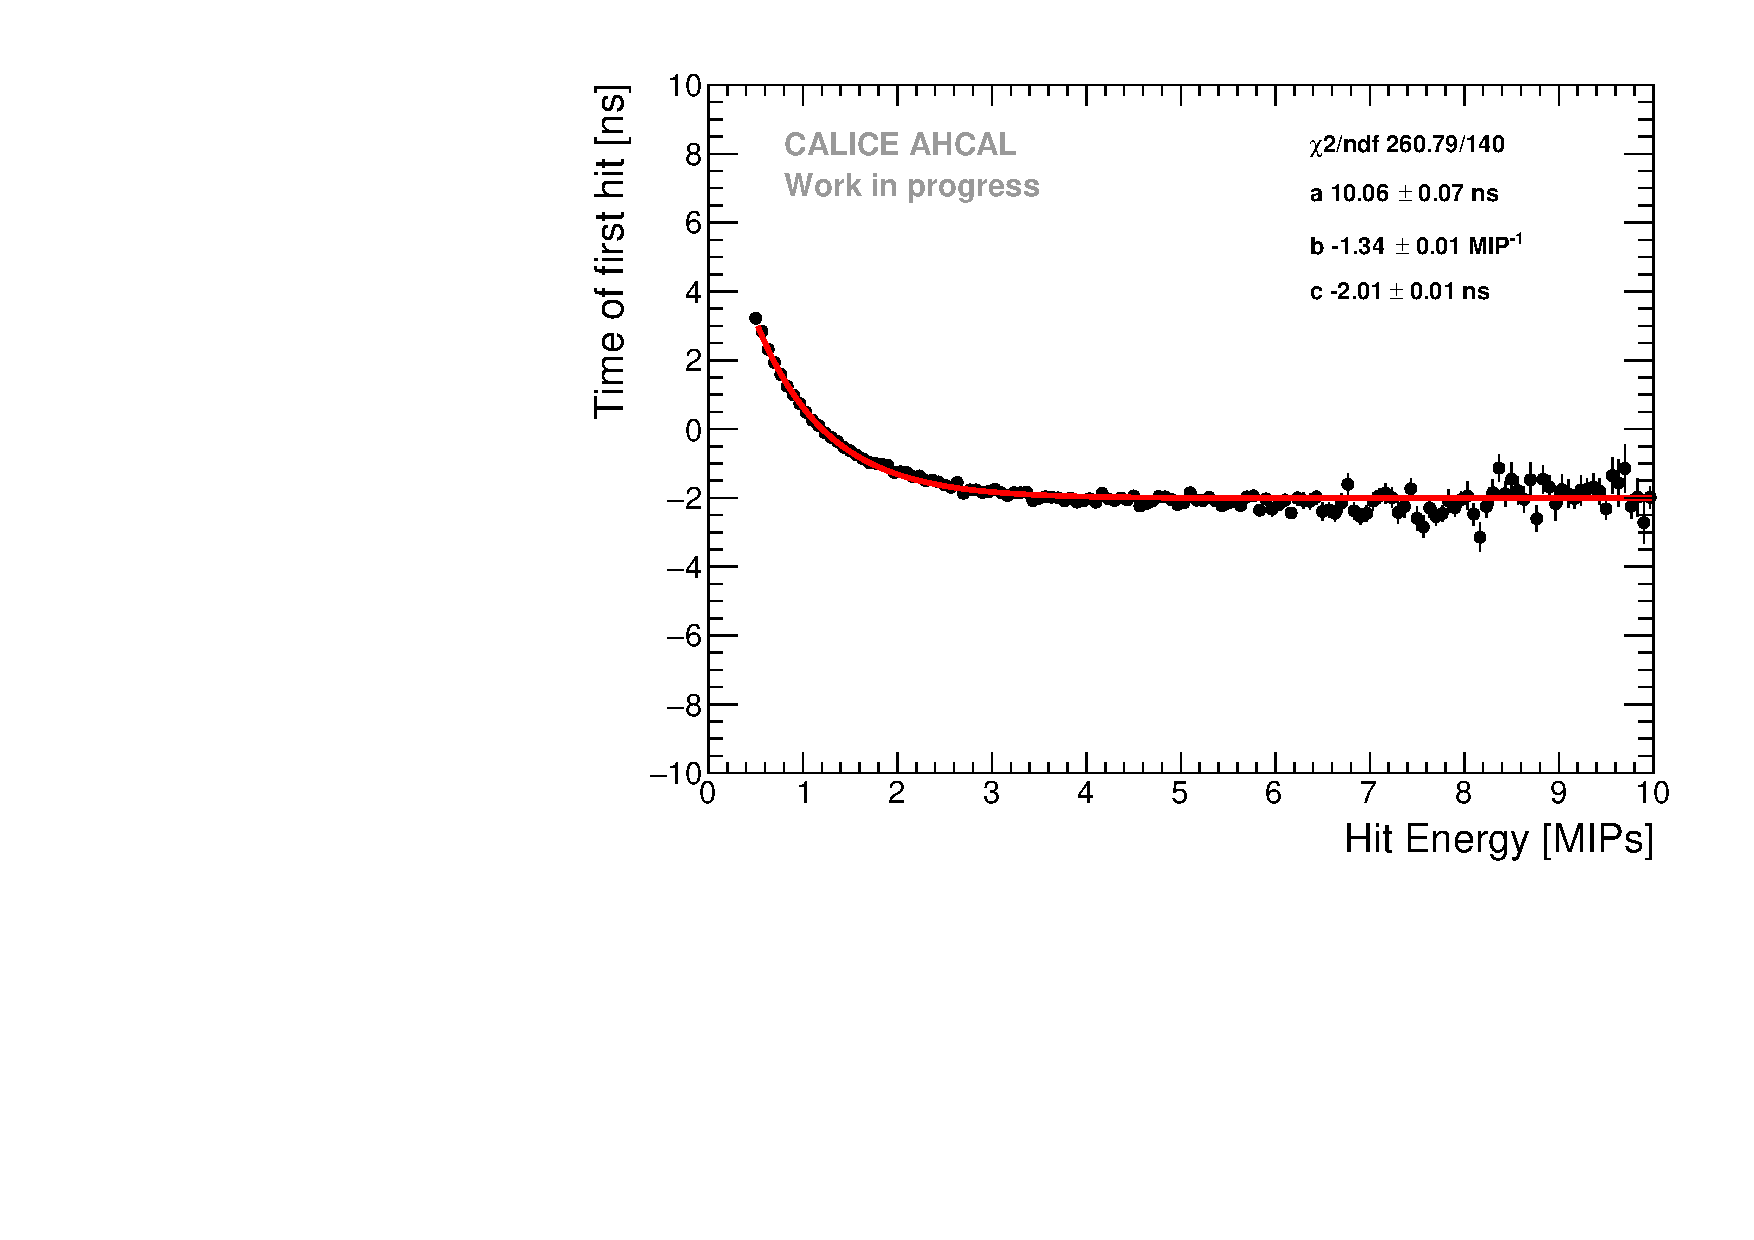
\includegraphics[width=1\textwidth]{../Thesis_Plots/Timing/Muons/Plots/TimeWalkProfile.pdf}
		\caption{}\label{fig:time_walk}
	\end{subfigure}
	\hfill
	\begin{subfigure}[t]{0.5\textwidth}
		\centering
		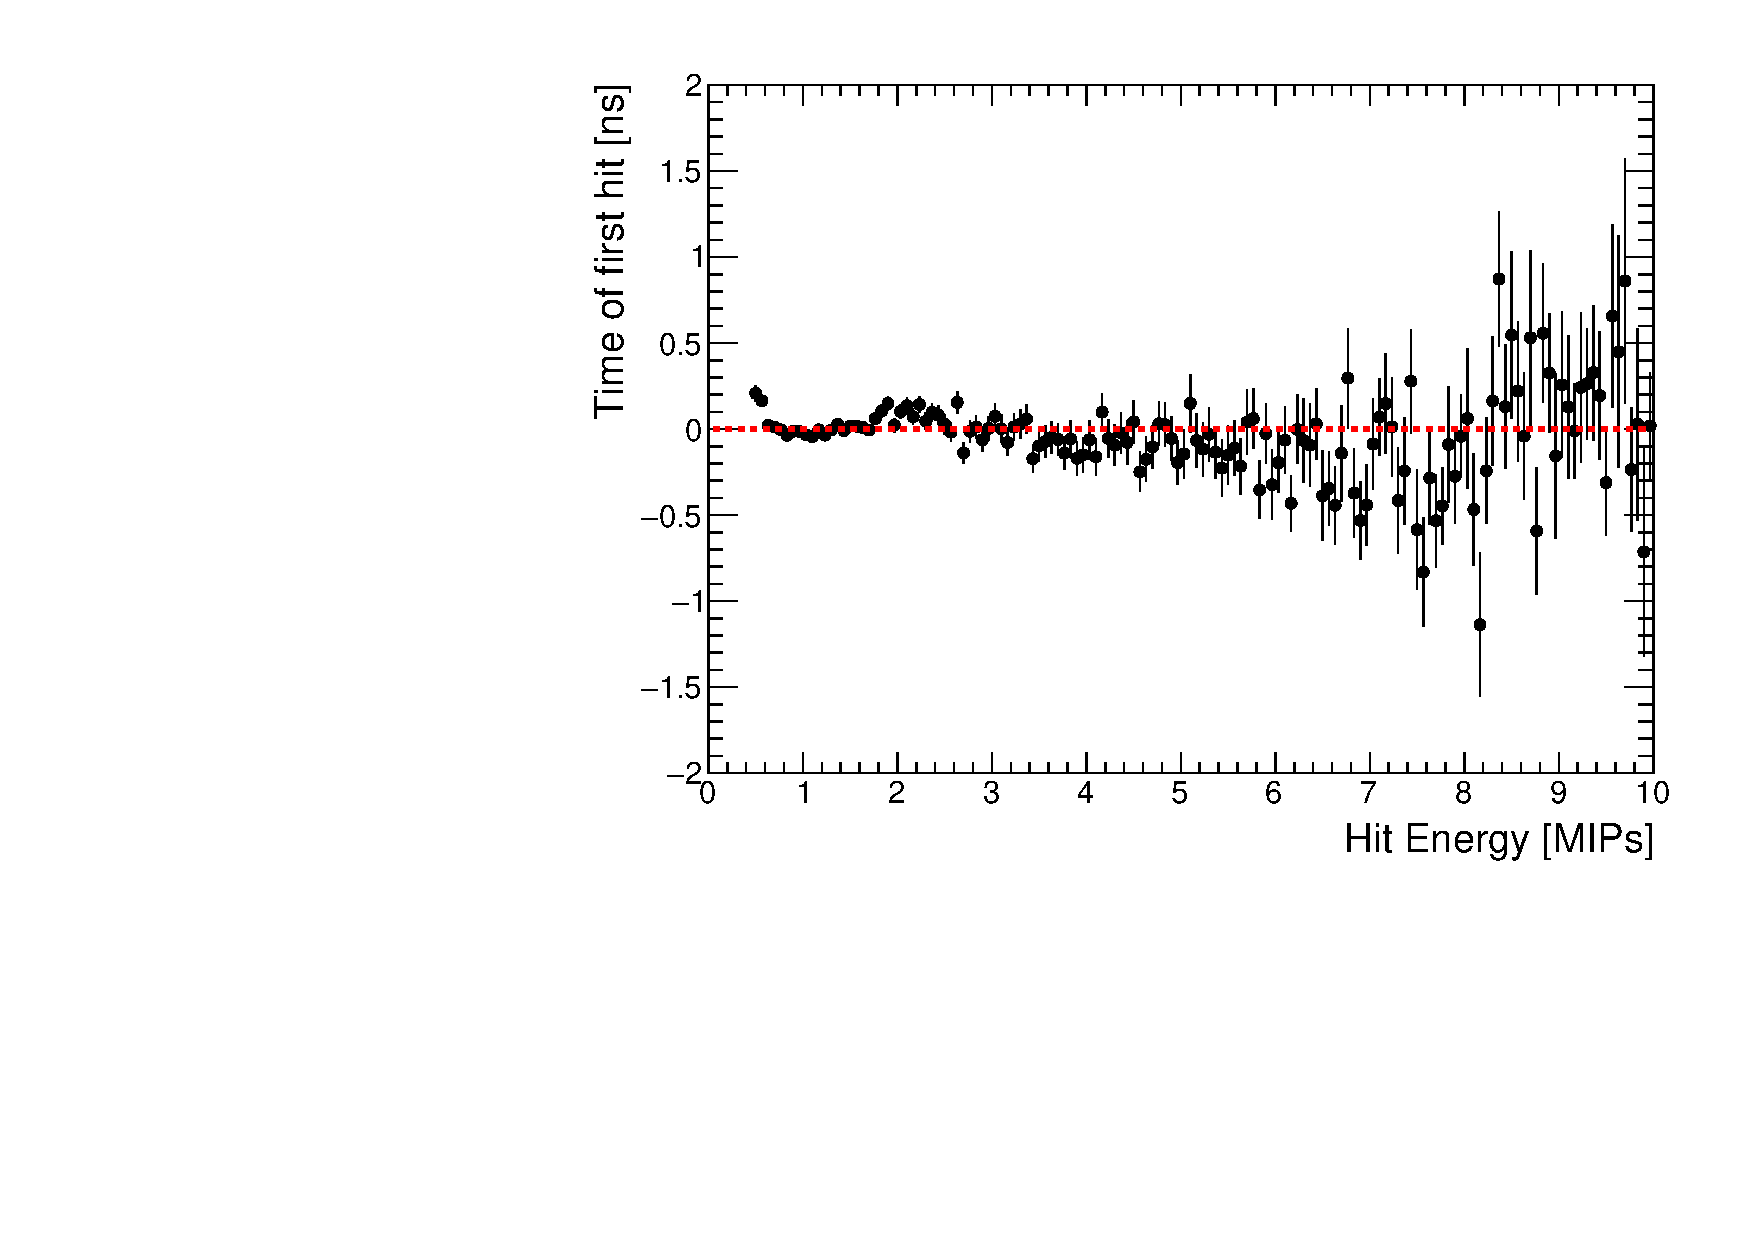
\includegraphics[width=1\textwidth]{../Thesis_Plots/Timing/Muons/Plots/TimeWalkProfile_Correction.pdf}
		\caption{}\label{fig:time_walk_corr}
	\end{subfigure}
	\caption{\subref{fig:time_walk}) Time of first hit as a function of the hit energy. A difference up to 6 ns is seen between small and large amplitudes. Time-walk correction extracted from data. The fit function is of the form $\text{A} \times e^{-\lambda{}x} + \text{B}$. \subref{fig:time_walk_corr}) Time of first hit as a function of the hit energy after correction showing a spread of less than 1 ns.}
\end{figure}

The correction is assumed to be the same for all the chips, independent of the position of the threshold of each chip, as hits are cut at 0.5 MIP. Thresholds of most of the chips were set to similar values and the threshold was set-up well below 0.5 MIP. It has been verified and no significant differences in the shape of the curve are seen between different chips. An exponential fit of the form $\text{A} \times e^{-\lambda{}x} + \text{B}$ is applied on the data to extract the parameters needed to correct the time walk effect as shown in figure \ref{fig:time_walk}. The residuals after correction, shown in figure \ref{fig:time_walk_corr}, are under one nanosecond.

\subsection{Time of first hit for muons after corrections}
\label{subsec:Muon_final}

After the time-walk correction, an improvement of around 3\% can be achieved on the time resolution of the AHCAL as shown in figure \ref{fig:timing_muons}. The figure \ref{fig:timing_reso_all_muons} shows the time resolution obtained for all the layers in the AHCAL. The obtained time resolution is around 5.2 ns RMS. The asymmetry of the distribution is taken into account in the simulation by parametrizing the time distribution with a double Gaussian function as shown in table \ref{table:time_res_sim}.

\begin{figure}[htbp!]
	\begin{subfigure}[t]{0.5\textwidth}
		\centering
		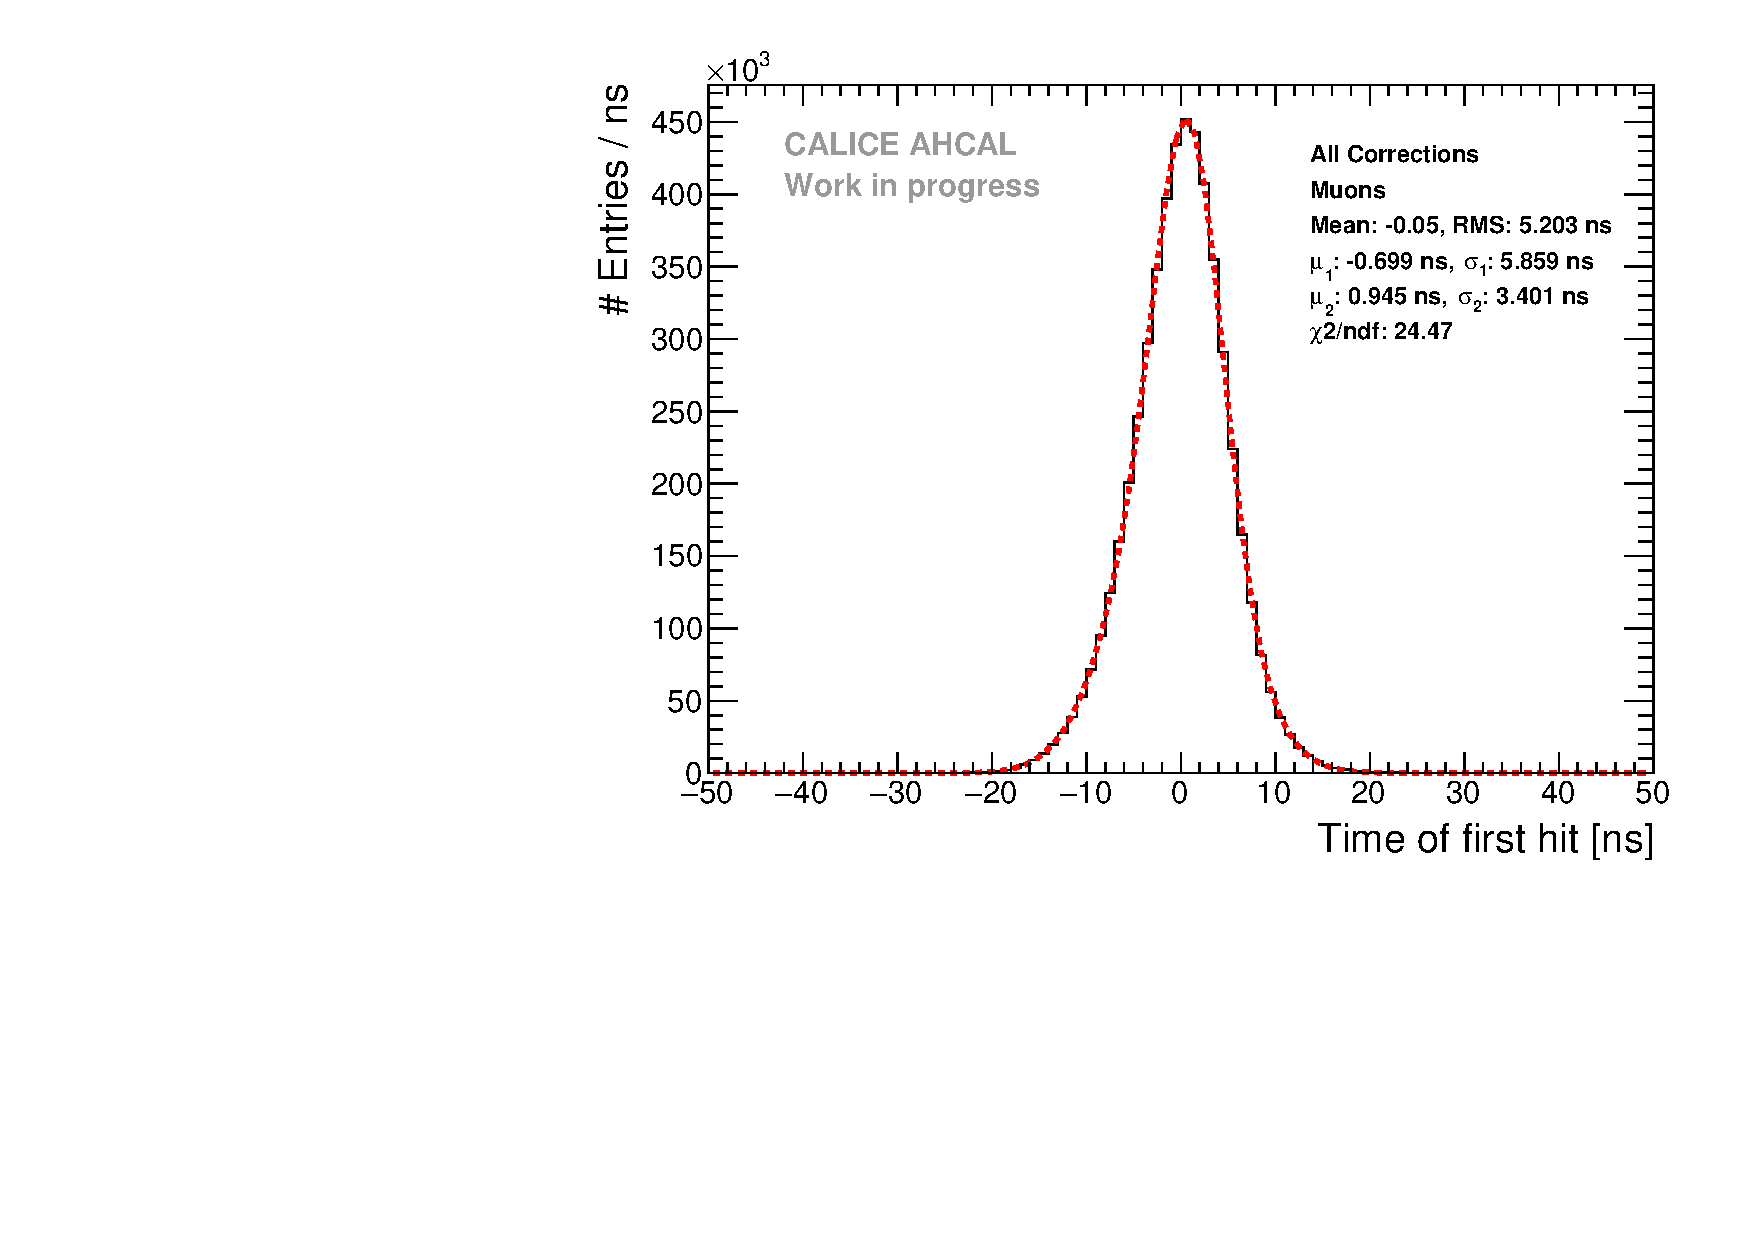
\includegraphics[width=1\textwidth]{../Thesis_Plots/Timing/Muons/Plots/Timing_AllLayers.pdf}
		\caption{}\label{fig:timing_muons}
	\end{subfigure}
	\hfill
	\begin{subfigure}[t]{0.5\textwidth}
		\centering
		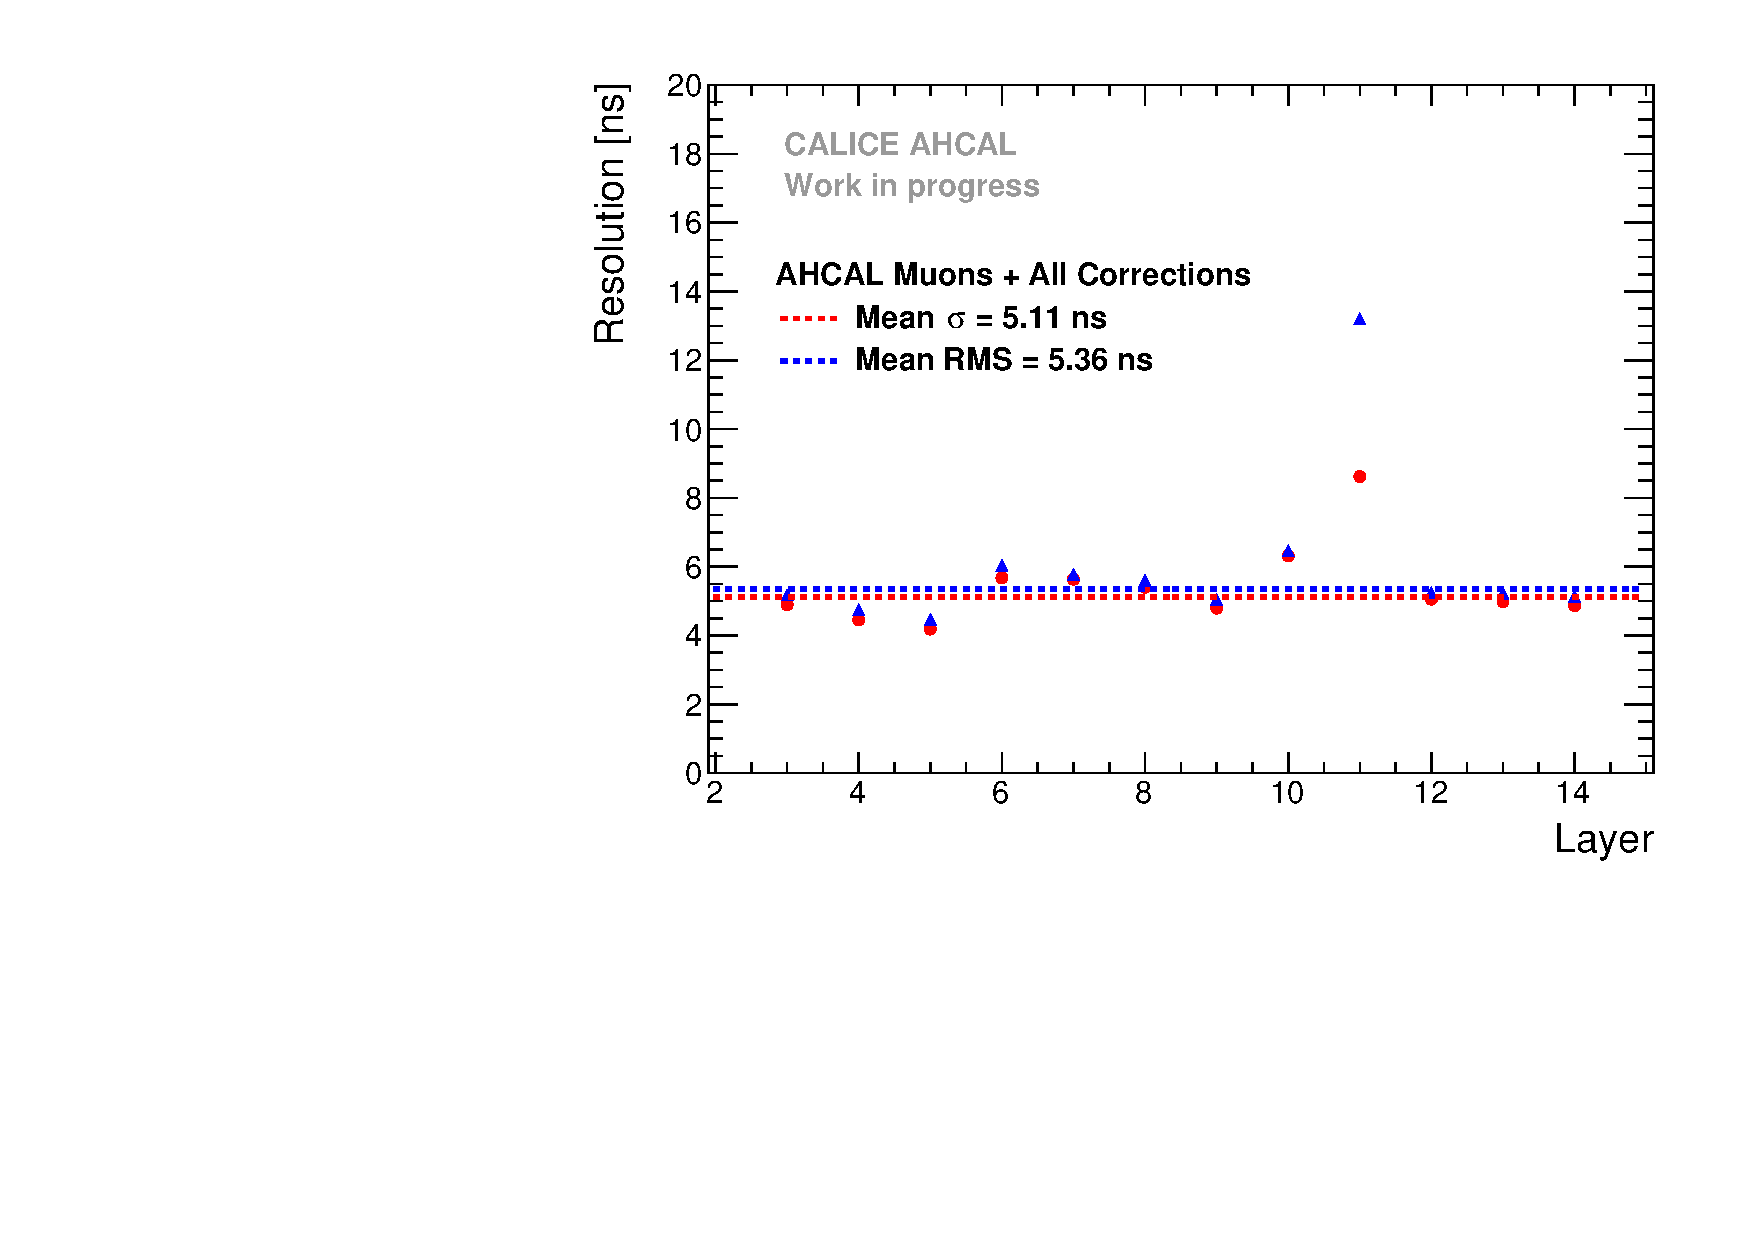
\includegraphics[width=1\textwidth]{../Thesis_Plots/Timing/Muons/Plots/ResolutionPerModule_AllCorrection.pdf}
		\caption{}\label{fig:timing_reso_all_muons}
	\end{subfigure}
	\caption{\subref{fig:timing_muons}) Time of the first hit for muons after all corrections excluding layer 11. The extracted parameters are then used to tune the simulation. \subref{fig:timing_reso_all_muons}) Time resolution obtained for each layer in the AHCAL. The mean RMS is 5.36 ns.}
\end{figure}

\begin{center}
	\rule{0.5\textwidth}{.4pt}
\end{center}

This chapter presented the timing calibration of the AHCAL with the recorded muon data. The TDC ramp slope determination, the calibration of the time reference and the different corrections applied to data have been explained. A timing resolution for the AHCAL of around 5 ns is achieved with muons.

Before investigating hadronic showers, the calibration must be cross-checked and the simulation must be validated. Electromagnetic showers are quasi-instantaneous and, in addition, they have a higher number of hits min the detector compared to muons as well as higher hit energies, and therefore are the perfect tool to perform the cross-check of the calibration. The cross-check of the calibration is discussed in the next chapter.
